\section{$\nu_e$ Exclusive Selections}
\label{sec:nueselection}
\par This section presents the two exclusive $\nu_e$ selections which are used in the low-energy analysis. We start with describing the common variables and tools leveraged by all $\nu_e$ selections in section~\ref{sec:nueselection:variables}. Next, the \npsel (sec.~\ref{sec:nueselection:1eNp}) and \zpsel (sec.~\ref{sec:nueselection:1e0p}) channel selections are presented, starting with a description of where the two selections branch off in sec.~\ref{sec:nueselection:inputs}. The $\nu_e$ inclusive selection, sensitive to a higher energy range, will be presented in a Sec.\ref{sec:nueselection:inclusive}.

\subsection{Variable definitions}
\label{sec:nueselection:variables}
\par This section describes the variables used in the $\nu_e$ selections to isolate features that are specific to events with final-state electrons. We split these variables in several categories according to the pertinence of the calorimetric or topological information used: Slice Variables, Shower, Track, Shower and Track, and Shower/Track-like  Classification Variables,  2nd Shower-Based $\pi^0$ Rejection Variables.  While table ~\ref{tab:variableSummary} summarizes all variables used with a brief description, variables that warrant a longer introduction are described below.

\par \noindent  \textbf{Slice Variables}: these variables describe general features of the reconstructed neutrino interaction or event.
\par \noindent  \textbf{Track Variables}: these variables describe the features of tracks objects.
\par \noindent \textbf{Shower Variables}:  these variables describe the features of shower objects.
\par \noindent \textbf{Shower-Track Distance Variables}: these variables are used to measure the separation in space between the leading shower and the leading track, for events where at least one track and one shower are present in the slice. 
\begin{itemize}
 \item[] \textbf{3D shower-track distance} (variable: \emph{tksh\_distance}).  This variable is the 3D distance between the shower start point and the reconstructed start point of the longest track in the slice. 
 \item[] \textbf{2D track-shower distance} (variable: \emph{trkshrhitdist2}) Due to mis-reconstruction in the 3D shower and track reconstruction, sometimes the 3D distance just defined (\emph{tksh\_distance}) is significantly smeared (up to several centimeters) even if the individual track and shower are correctly clustered. These factors decreases the track-shower separation of $\nu_e$ interactions therefore reducing the $e-\gamma$ separation power achievable. To overcome this failure specific to the 3D reconstruction, a new quantity is calculated with 2D information from the collection plane defined as the smallest 2D distance between any hits associated with the shower candidate and any hits associated with the proton candidate. This variable is therefore complementary to the quantity \emph{tksh\_distance}.
\end{itemize}



\par \noindent \textbf{Shower/Track-like  Classification Variables}: The first step in track-shower classification relies on the topological score reconstructed by Pandora (variable: \emph{shr\_score}), which utilizes inputs such as the PCA component of 3D space-points to classify PFParticles. Nonetheless, this classification is not sufficient to obtain the track-shower separation needed. To improve on this, additional variables which leverage different aspects of shower topologies are devised:

\begin{itemize}

    \item[] \textbf{Shower Track-Fitted Fraction} (variable: \emph{trfit}, figure~\ref{fig:nue:variables:trkfit}) This quantity is the fraction of the 3D spacepoints in a shower object that are successfully fit with the shower track-fitter algorithm. Tracks, comprised of a single contiguous segment, will be entirely fit, leading to a fraction of 1. Showers, with several branches and split charge deposition segments, will have a fraction that is less then one.
    \item[] \textbf{Shower Sub-Clusters} (variable: \emph{subcluster}, figure~\ref{fig:nue:variables:subcluster}) This quantity leverages the fact that EM showers are often comprised of several branches isolated by gaps caused by photons propagating through the detector medium. The variable is calculated by counting the number of isolated 2D segments of charge associated to reconstructed showers. This quantity is a sum of such clusters from all three planes.
    \item[] \textbf{Moliere ``Angle''} (variable: \emph{shrmoliereavg}, figure~\ref{fig:nue:variables:dedx}) This quantity aims to characterize the profile of reconstructed EM showers. It is computed using 3D spacepoints. For each 3D spacepoint, the angle between the shower's direction and the spacepoint is calculated. The average of all such angles is used as the variable.
    \item[] \textbf{dE/dx Variables} (variables: \emph{shr\_tkfit\_2cm\_dedx\_\{U,V,Y\}} and \emph{shr\_tkfit\_gap10\_dedx\_\{U,V,Y\}} )  These variables are computed using calorimetric information from each plane separately. The two different variables are calculated as the median d$E$/d$x$ computed over some segment of a shower's trunk. The two segments used are the first two centimeters, and the range [1,5] cm, respectively. Two reasons justify the us of both these variables. Firstly, there are cases where the first few hits of a shower merge activity from short protons, causing a large d$E$/d$x$ which hampes the ability to identify the shower as an electron. These cases are particularly relevant as backgrounds for the 1$e$0$p$ channel. Secondly, in case of photon showers, d$E$/d$x$ becomes more and more MIP-like as one moves further along the shower, especially at low energy (see figure~\ref{fig:dedxgammas:dist}).
\end{itemize}{}

\begin{figure}[H] 
\begin{center}
    \begin{subfigure}[b]{0.3\textwidth}
    \centering
    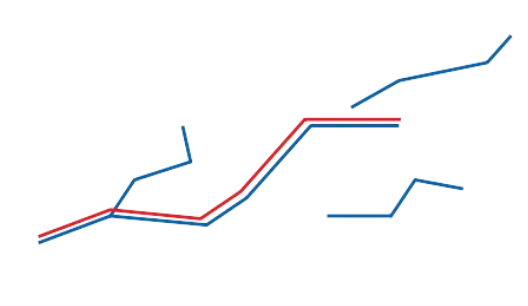
\includegraphics[width=1.00\textwidth]{nueselection/variables/trkfit.png}
    \caption{\label{fig:nue:variables:trkfit} ``trkfit'' variable }
    \end{subfigure}
    \begin{subfigure}[b]{0.3\textwidth}
    \centering
    
\includegraphics[width=1.00\textwidth]{nueselection/variables/nbranch.png}
    \caption{\label{fig:nue:variables:subcluster} ``subcluster'' variable }
    \end{subfigure}
    \begin{subfigure}[b]{0.3\textwidth}
    \centering
    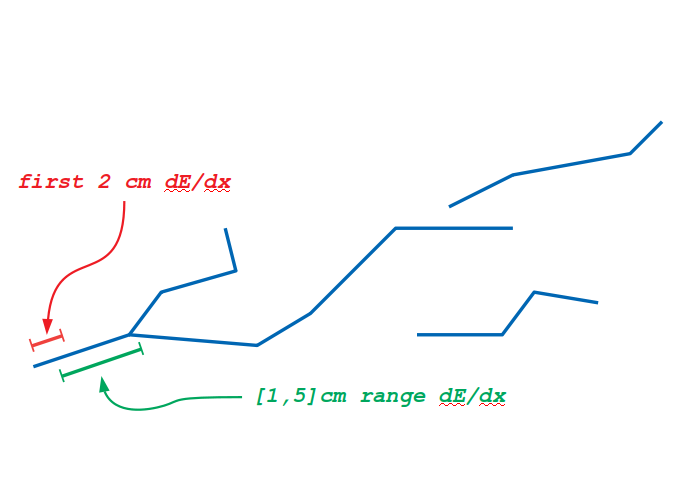
\includegraphics[width=1.00\textwidth]{nueselection/variables/dedx.png}
    \caption{\label{fig:nue:variables:dedx} d$E$/d$x$ variables }
    \end{subfigure}
\caption{\label{fig:nue:presel:eff} Additional shower variables defined by the analysis to improve track-shower separation.}
\end{center}
\end{figure}

\par \noindent  \textbf{Second Shower Based $\pi^0$ Rejection Variables}: %Often, one of the two EM $\gamma$ showers in $\pi^0$ events is not fully reconstructed by Pandora. In many cases, these second $\gamma$ showers are correctly identified by Pandora as belonging to the neutrino slice (reconstructed in 2D), but never fully reconstructed in 3D (see fig.~\ref{fig:nue:variables:secondshowerevd}).
Pandora's reconstruction of events containing $\pi^0$ is often imperfect. In many cases, both EM $\gamma$ showers are correctly identified as belonging to the same neutrino slice (reconstructed in 2D), but one of the showers is not fully reconstructed in 3D (see fig.~\ref{fig:nue:variables:secondshowerevd}).

To improve on our $\pi^0$ rejection, we build several variables storing information associated to the largest 2D cluster in the slice on each plane. At the moment, only collection-plane variables are used. The variables, shown graphically in figure~\ref{fig:nue:variables:secondshower}, are described in table ~\ref{tab:variableunSummary}. In the example event of figure~\ref{fig:nue:variables:secondshowerevd}, these quantities are computed for the circles black cluster of charge which represents a missed photon in the $\pi^0$ reconstruction.

\begin{figure}[H] 
\begin{center}
    \begin{subfigure}[b]{0.35\textwidth}
    \centering
    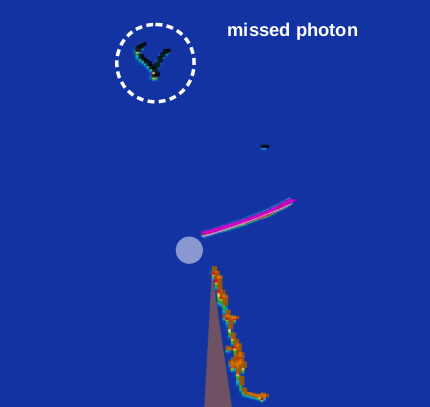
\includegraphics[width=1.00\textwidth]{nueselection/variables/secondshowerevd.png}
    \caption{\label{fig:nue:variables:secondshowerevd} unclustered shower }
    \end{subfigure}
    \begin{subfigure}[b]{0.35\textwidth}
    \centering
    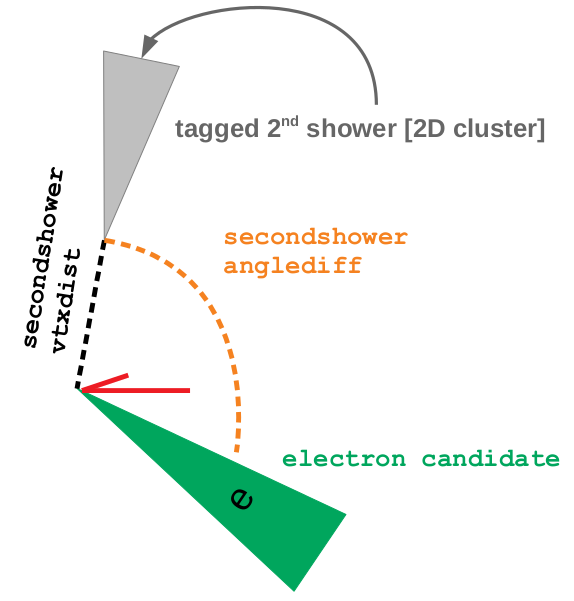
\includegraphics[width=1.00\textwidth]{nueselection/variables/secondshower.png}
    \caption{\label{fig:nue:variables:secondshower}second-shower variables }
    \end{subfigure}
\caption{\label{fig:nue:variables:secondshower} Visual representation of the second shower based $\pi^0$ rejection variables. Left: example event where the second shower in a $\pi^0$ event is clustered in 2D (black hits) but not fully reconstructed in 3D. Right: reconstructed variables associated to the 2nd-shower search. The gray cone in the image represents the black cluster on the left image, for which only 2D information is accessible.}
\end{center}
\end{figure}

\begin{table}[ht]
\caption{\label{tab:variableSummary} Summary of the definition for the variables used in the analysis.}
\centering
\begin{tabular}{ m{0.08\textwidth} | m{0.25\textwidth} | m{0.6\textwidth}  }
Category & Variable Name & Description  \\
\hline

\multicolumn{1}{l|}{} & \emph{nslice} &  Number of neutrino slices identified by the \emph{SliceID}. Values are  0 or 1.\\  \cline{2-3}
\multicolumn{1}{l|}{} & \emph{reco\_nu\_vtx\_sce\_\{x,y,z\}} & Reconstructed neutrino interaction vertex in (x,y,z) coordinates. The space charged correction is applied.  \\  \cline{2-3}
\multicolumn{1}{l|}{} & \emph{n\_showers\_contained} & Number of showers with a starting point within the fiducial volume. \\  \cline{2-3}
\multicolumn{1}{l|}{} & \emph{n\_tracks\_contained} & Number of tracks fully contained in the fiducial volume.  \\  \cline{2-3}
\multicolumn{1}{l|}{} & \emph{contained\_fraction} & Hits in PFParticles contained in the fiducial volume over the total number of clustered hits in the slice.  \\  \cline{2-3}
\parbox[t]{2mm}{\multirow{4}{*}{\rotatebox[origin=c]{90}{Slice}}} & \emph{hits\_ratio} & Ratio between hits from showers and total number of hits in the slice. \\  \cline{2-3}
\multicolumn{1}{l|}{} & \emph{CosmicIP} & Closest distance between shower start and space points associated to tracks flagged as cosmics. \\  \cline{2-3}
\multicolumn{1}{l|}{} & \emph{crtveto} & Boolean variable checking if the event passes the CRT veto. \\  \cline{2-3}
\multicolumn{1}{l|}{} & \emph{\_closestNuCosmicDist} &  3D distance between the reconstructed neutrino vertex and the closest CRT-tagged cosmic track. \\  \cline{2-3}
\multicolumn{1}{l|}{} & \emph{slclustfrac} & Fraction of hits in the slice that are fully reconstructed to 3D particles. \\  \cline{2-3}
\multicolumn{1}{l|}{} & \emph{nObjHits\_\{U,V,Y\}} & Number of hits associated with the object on each plane.\\  \cline{2-3}
\hline

\hline
\multicolumn{1}{l|}{} & \emph{pfp\_generation} & The generation of the PFParticle according to Pandora: the neutrino has generation 1, it's direct daughters 2, and further decay products 3 or higher.\\  \cline{2-3}
\multicolumn{1}{l|}{} & \emph{trkpid}  &  Proton-muon LLR particle identification. \\  \cline{2-3}
\parbox[t]{2mm}{\multirow{4}{*}{\rotatebox[origin=c]{90}{Track, Shower and Their Separation}}}  & \emph{shr\_energy\_tot\_cali}  & Sum  of  the  energy  of  the  calibrated  showers  (in  GeV). Used  only  at pre-selection as a ``Michel veto”.\\  \cline{2-3}
\multicolumn{1}{l|}{} & \emph{shr\_score} & Pandora  SVM track/shower score for the leading shower.\\  \cline{2-3}
\multicolumn{1}{l|}{}  & \emph{tksh\_distance}  & Distance between leading shower and longest track start points.\\  \cline{2-3}
\multicolumn{1}{l|}{} & \emph{tksh\_angle}  & Angle  between  leading  shower   and  longest  track directions.\\  \cline{2-3}
\multicolumn{1}{l|}{} & \emph{merge\_bestdist}  & Distance between shower start point and track start (or end) point for the track in the slice that best matches the direction of the shower.\\  \cline{2-3}
\multicolumn{1}{l|}{} & \emph{trfit} & Fraction of the 3D spacepoints successfully fitted with the shower track-fitter algorithm. \\  \cline{2-3}
\multicolumn{1}{l|}{} & \emph{subcluster} & Number of isolated 2D segments of charge associated to a reconstructed shower on all three planes  \\  \cline{2-3}
\multicolumn{1}{l|}{} & \emph{shrmoliereavg} &  Average angle between the shower’s direction and its 3D spacepoints.    \\ \cline{2-3}
\multicolumn{1}{l|}{} & \emph{shr\_tkfit\_gap10\_dedx\_\{U,V,Y\}}  & Median dE/dx computed over the [1,5] cm of the shower’s  trunk. \\ \cline{2-3}
\multicolumn{1}{l|}{} & \emph{shr\_tkfit\_2cm\_dedx\_\{U,V,Y\}}  & Median dE/dx computed  over  the first 2 cm of the shower’s  trunk. \\ \cline{2-3}
\multicolumn{1}{l|}{} & \emph{shower\_vtx\_dist} & Distance between the shower start and the neutrino vertex.\\ \cline{2-3}
\multicolumn{1}{l|}{} & \emph{ismerged} & Check if a proton is merged at the beginning of a shower.\\ \cline{2-3}
\hline
\hline
\multicolumn{1}{l|}{} & \emph{secondshower\_Y\_nhit} & Number of hits in the collection plane of the largest cluster associated to the  recovered 2nd shower  \\  \cline{2-3}
\parbox[t]{2mm}{\multirow{4}{*}{\rotatebox[origin=c]{90}{Second Shower}}}  & \emph{secondshower\_Y\_dot} &  Dot product between the vector connecting the vertex to the closest hit in cluster and the charge-weighted cluster direction w.r.t. closest hit in cluster \\  \cline{2-3}
\multicolumn{1}{l|}{} & \emph{anglediff\_Y} & 2D angle difference in the collection plane between the 2nd shower and the 1st shower cluster  (cluster direction defined as charge-weighted direction of cluster w.r.t. vertex) \\ \cline{2-3}
\multicolumn{1}{l|}{} & \emph{secondshower\_Y\_vtxdist} & 2D distance from vertex for the largest 2D cluster associated to the  recovered 2nd shower in the collection plane \\
\hline
\end{tabular}
\label{tab:variableSummary}
\end{table}

\clearpage

\subsection{Input to \npsel and \zpsel selections and channel orthogonality }
\label{sec:nueselection:inputs}

The \npsel and \zpsel selections rely on a common pre-selection which requires the presence of at least one reconstructed and contained EM shower (figure~\ref{fig:nue:presel:nshower}) with reconstructed energy above 70 MeV (figure~\ref{fig:nue:presel:shrenergy}). This second cut acts as a Michel-electron veto, since the majority of events which do not pass this cut are associated with cosmic or $\nu_{\mu}$ induced $\mu \rightarrow e$ Michel electrons. 
In addition, as a containment cut we require that more than 90\% of clustered hits in the slice are associated to PFParticles that are  contained  in the fiducial volume.
The two selections are subsequently split: we require the presence of at least one fully contained track for the \npsel channel and the absence of fully contained tracks for the \zpsel channel.

\begin{figure}[H] 
\begin{center}
    \begin{subfigure}[b]{0.3\textwidth}
    \centering
    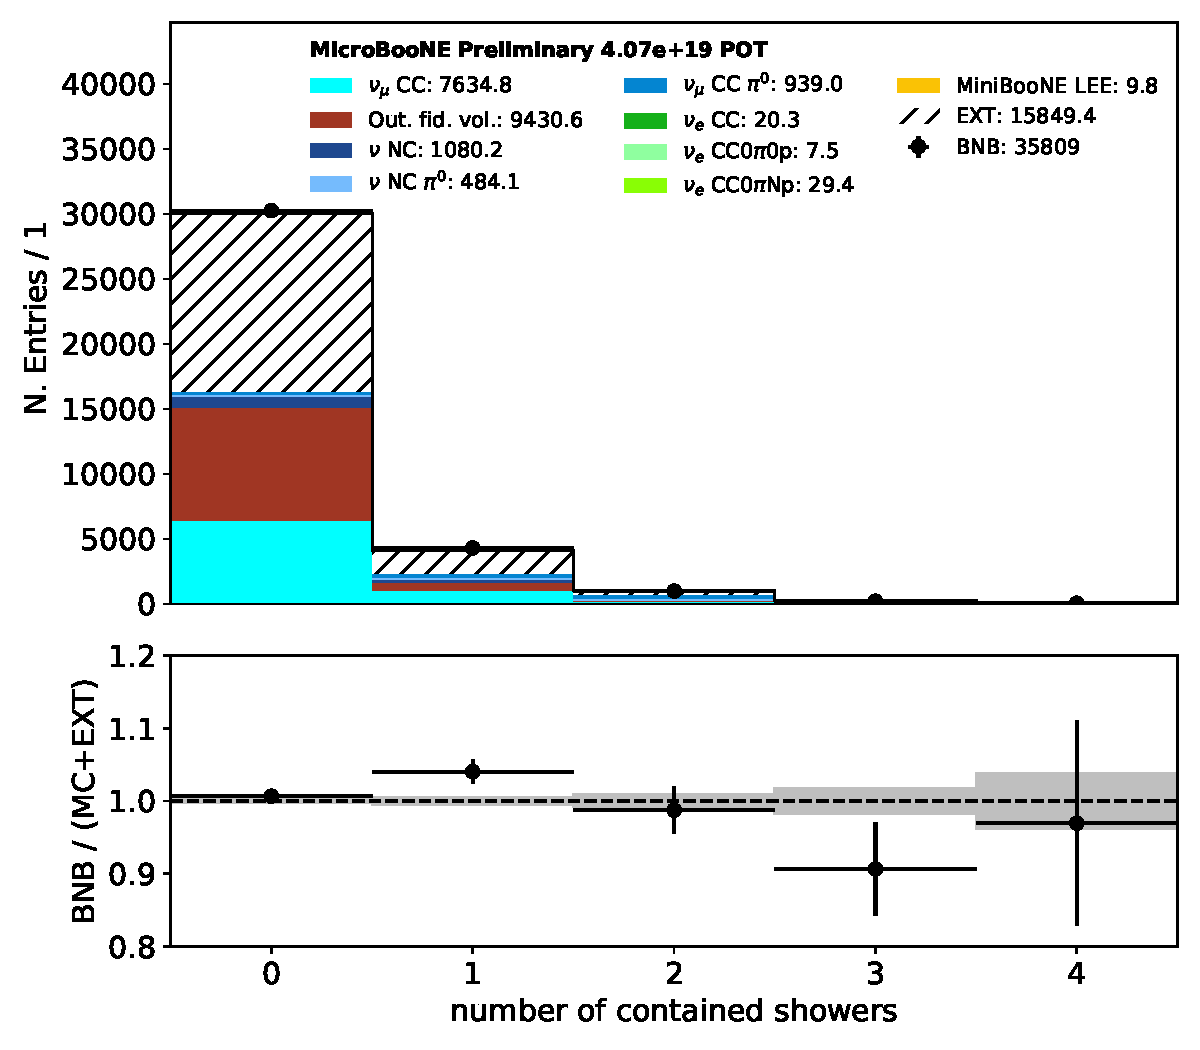
\includegraphics[width=1.00\textwidth]{nueselection/n_showers_contained_01132020_RUN1.pdf}
    \caption{\label{fig:nue:presel:nshower} Contained showers}
    \end{subfigure}
    \begin{subfigure}[b]{0.3\textwidth}
    \centering
    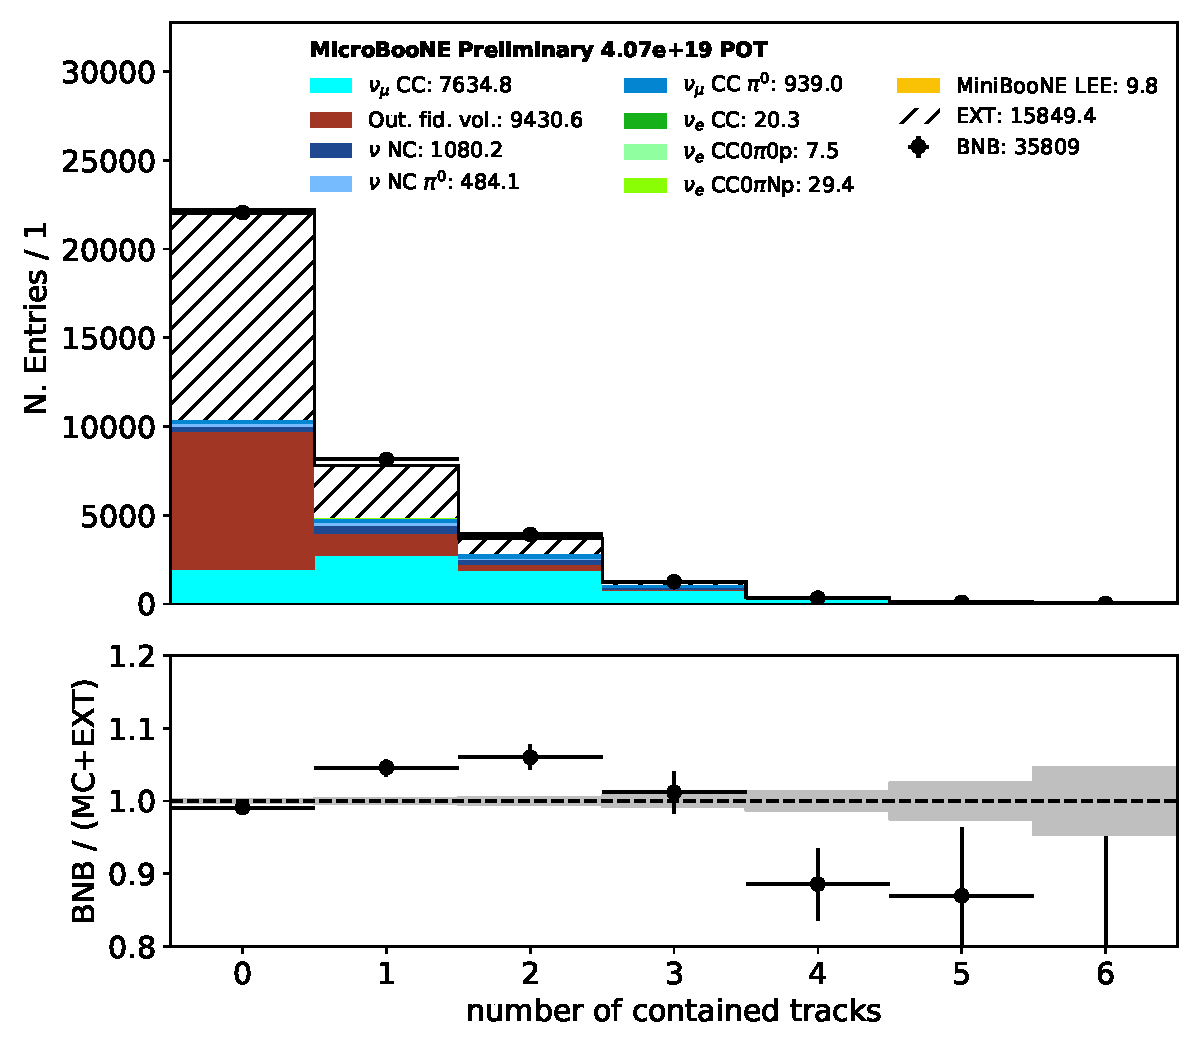
\includegraphics[width=1.00\textwidth]{nueselection/n_tracks_contained_01132020_RUN1.pdf}
    \caption{\label{fig:nue:presel:ntrack} Contained tracks}
    \end{subfigure}
    \begin{subfigure}[b]{0.3\textwidth}
    \centering
    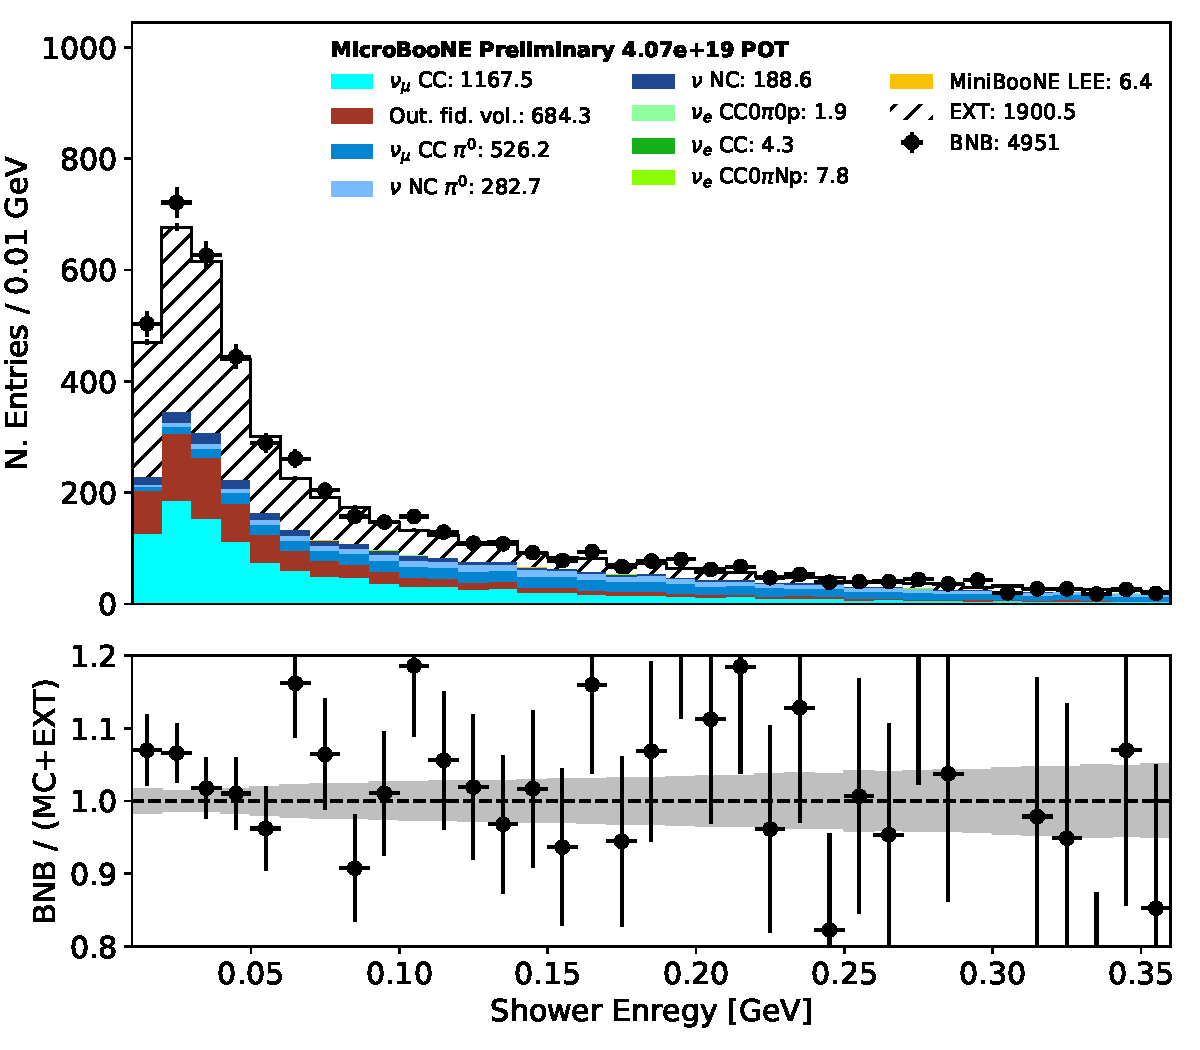
\includegraphics[width=1.00\textwidth]{nueselection/shr_energy_tot_cali_01132020_RUN1.pdf}
    \caption{\label{fig:nue:presel:shrenergy} Shower energy}
    \end{subfigure}
\caption{\label{fig:nue:presel}Variables input to the common $\nu_e$ N$p$ and 0$p$ pre-selection.}
\end{center}
\end{figure}

\begin{comment}
\par The efficiencies of the 1$e$N$p$ and 1$e$0$p$ channels at the point where the selections diverge are shown in figure~\ref{fig:nue:presel:eff}. Efficiencies are presented as a function of true neutrino energy (fig.~\ref{fig:nue:presel:eff:nu}), proton KE (fig.~\ref{fig:nue:presel:eff:proton}), and electron energy (fig.~\ref{fig:nue:presel:eff:elec}). Each plot shows in black the efficiency for the common pre-selection (before requirements on protons are imposed) relative to all intrinsic $\nu_e$ events. The efficiencies for the  1$e$N$p$ and 1$e$0$p$ selections relative to true N$p$ and 0$p$ events are shown in blue and red respectively.
Shaded histograms in red and blue show the stacked truth-level distributions for N$p$ and 0$p$ events for the variables being plotted. It is important to observe that the reconstruction efficiency for 1$e$N$p$ events is significantly lower then that of 1$e$0$p$ events at this pre-selection stage. This is caused by the additional requirement of the presence of a proton-like track in the final state. The strong energy dependence for the efficiency in tagging protons is shown in figure~\ref{fig:nue:presel:eff:proton}. While requiring the presence of a final-state proton lowers the efficiency, this requirement has a significant impact on the selection's ultimate purity.

\begin{figure}[H] 
\begin{center}
    \begin{subfigure}[b]{0.3\textwidth}
    \centering
    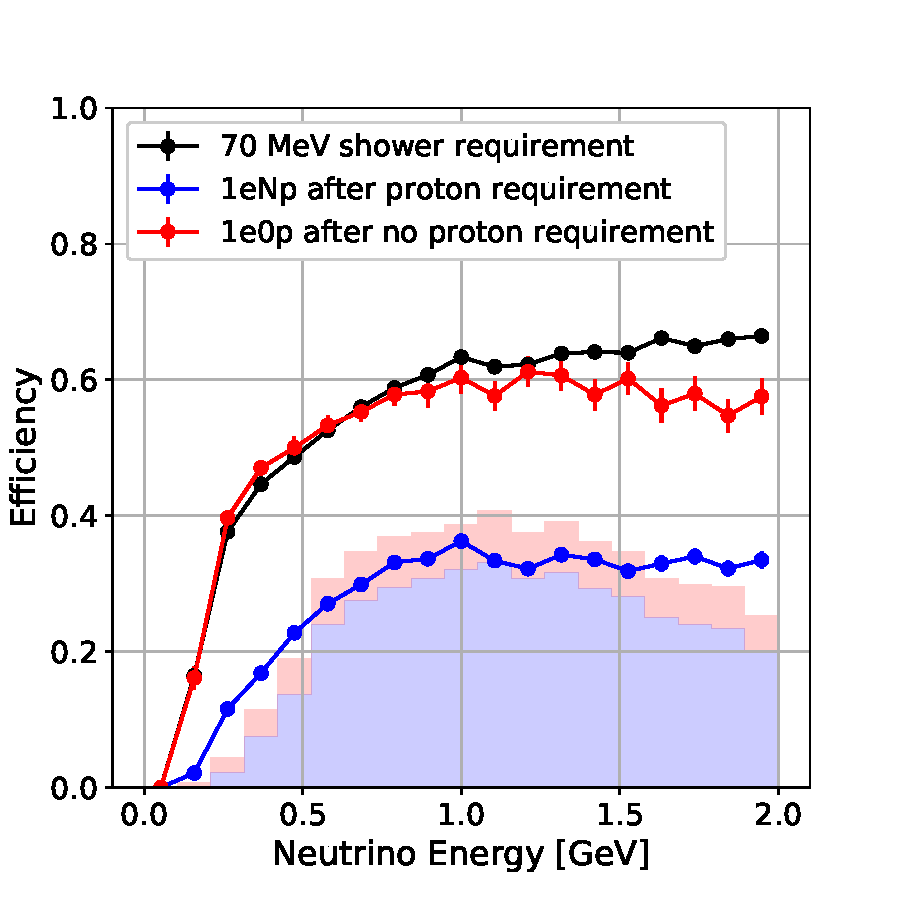
\includegraphics[width=1.00\textwidth]{nueselection/nu_RUN1.pdf}
    \caption{\label{fig:nue:presel:eff:nu} }
    \end{subfigure}
    \begin{subfigure}[b]{0.3\textwidth}
    \centering
    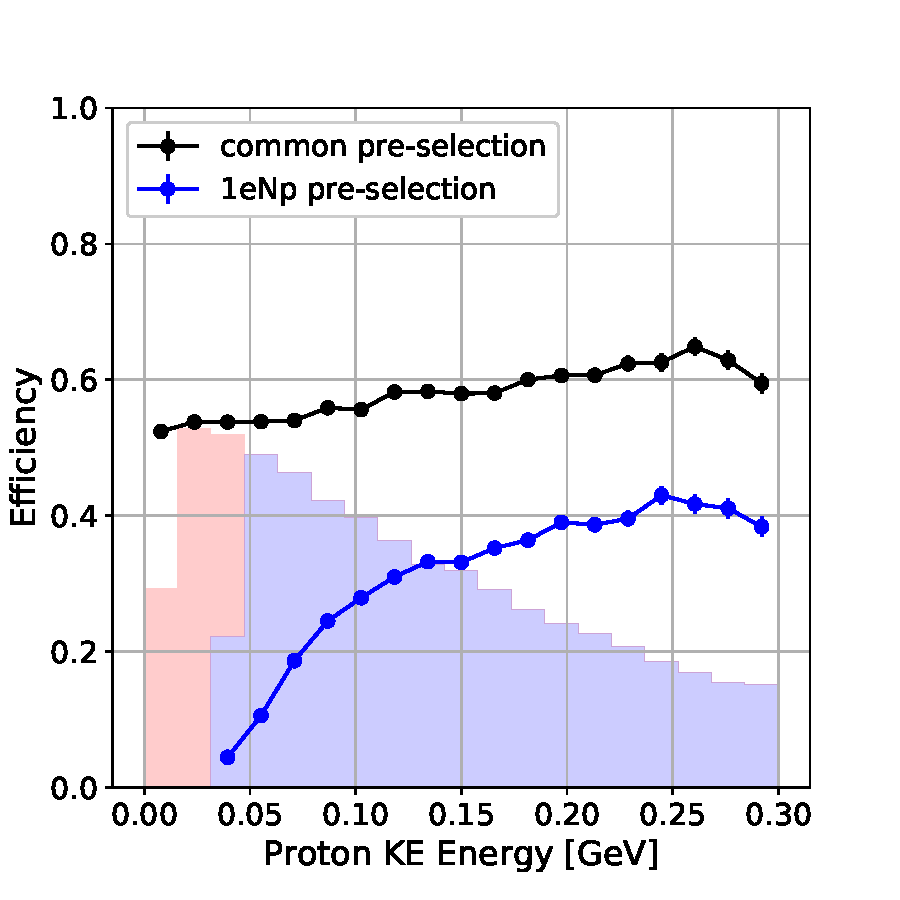
\includegraphics[width=1.00\textwidth]{nueselection/proton_RUN1.pdf}
    \caption{\label{fig:nue:presel:eff:proton} }
    \end{subfigure}
    \begin{subfigure}[b]{0.3\textwidth}
    \centering
    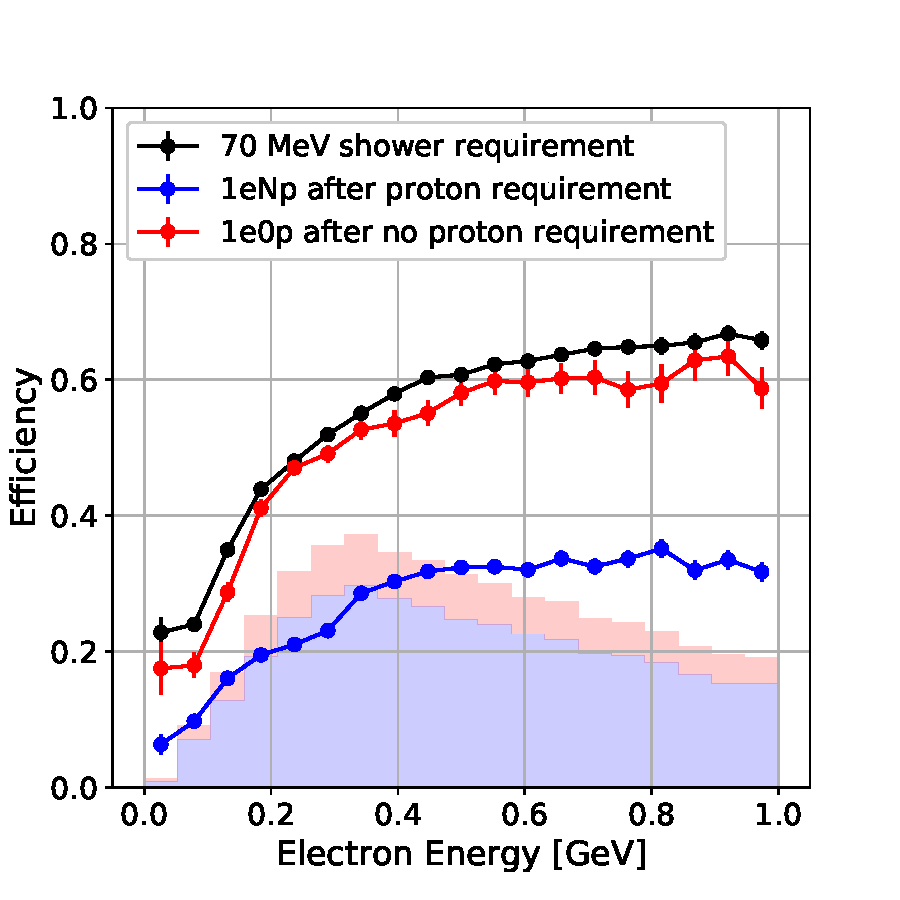
\includegraphics[width=1.00\textwidth]{nueselection/elec_RUN1.pdf}
    \caption{\label{fig:nue:presel:eff:elec} }
    \end{subfigure}
\caption{\label{fig:nue:presel:eff} $\nu_e$ pre-selection efficiencies split by final-state topology as a function of different truth variables. }
\end{center}
\end{figure}
\end{comment}{}

\subsection{\npsel Channel}
\label{sec:nueselection:1eNp}

The \npsel channel is the most sensitive to the MiniBooNE eLEE signal as it contains a large fraction of the signal events and allows for selection requirements based both on showers and tracks. Since $\nu_e$ charge-current interactions are O(1\%) in the BNB and a large cosmic background is present, a high-purity selection is needed to achieve a sizeable signal sensitivity; the necessary trade-off is that the final signal efficiency will be low.

The section is organized as follows. We first define a set of minimal requirements (``pre-selection") to obtain a high statistics sample used to monitor the data-MC agreement of the selection variables;
the events at the pre-selection stage are dominated by cosmic and neutrino backgrounds. We then define two alternative selections, one based on a simple box-cut approach and one on boosted decision trees (BDT); the BDT approach is expected to be the most sensitive, while box-cuts provide a robust reference selection. Finally, we compare all presented selections in terms for their signal efficiency and purity.

Two updates to the selection have been included since opening the far-sideband data for this analysis. They consist of a series of ``recovery'' algorithms which aim to re-interpret event information for events that fail the selection due to mis-reconstruction, as well as two cut updates at pre-selection stage. The recovery algorithms aim to mitigate reconstruction failures which occur largely at high-energy and do not impact the analysis at low energy. The most common such failure is associated to events where the electron is split in two reconstructed showers, which are recovered through a re-interpretation of the event as a one-shower topology. These algorithms are described in detail in sec.~\ref{sec:sideband:recovery}. The two minor cut updates, which also have no noticeable impact at low energy, are described in sec.~\ref{sec:sideband:newcuts:shrtrklen}
 and~\ref{sec:sideband:newcuts:nhits}. The contents of this chapter inclue and reflect these updates.
 
\subsubsection{Preselection}

We define a \npsel preselection by adding a requirement of at least one contained track on top of the common \nue preselection defined in Sec.~\ref{sec:nueselection}. 
The \npsel preselection is a minimum set of cuts that guarantees that all selection variables can be defined; the list of requirements can be found in Table~\ref{tab:1eNp:presel}.

\begin{table}[h!]
\centering
\setlength{\tabcolsep}{10pt}
\renewcommand{\arraystretch}{1.25}
 \begin{tabular}{| c | c |} 
 \hline
 Cut goal & Cut definition \\
 \hline\hline
Cosmic rejection & nslice = 1 \\
 \hline
\multirow{2}{*}{Signal~topology} & n\_tracks\_contained $>$ 0 \\
 & n\_showers\_contained $>$ 0 \\
 \hline
Containment & contained\_fraction $>$ 0.9 \\
 \hline
Michel rejection & shr\_energy\_tot\_cali $>$ 0.07 GeV \\
 \hline
 \end{tabular}
 \caption{\label{tab:1eNp:presel} Preselection requirements for the \npsel selection.}
\end{table}

The relative fraction of EXT events at this stage is roughly 25\%, so we can look at all selection variables in data and MC in a neutrino-dominated sample with the open Run1 and Run3 data sets. We typically see very good agreement, which rules out major problems related to POT-scaling, detector modeling, and flux and cross-section modeling. 
%The reader should keep in mind that current data-mc comparisons do not include a rescaling of the $\pi^0$ normalization, and that resolving discrepancies in $\pi^0$ normalization described in section~\ref{sec:sideband:pi0} will impact the final level of data-mc agreement. 
The full list of plots can be found in Appendix~\ref{app:nuepresel}. Figure~\ref{fig:1eNp:prsel} shows the level of agreement for the reconstructed neutrino energy variable after pre-selection. 

\begin{figure}[ht]
\begin{center}
% p-values: reco_e 0.3105 0.9905 0.8121
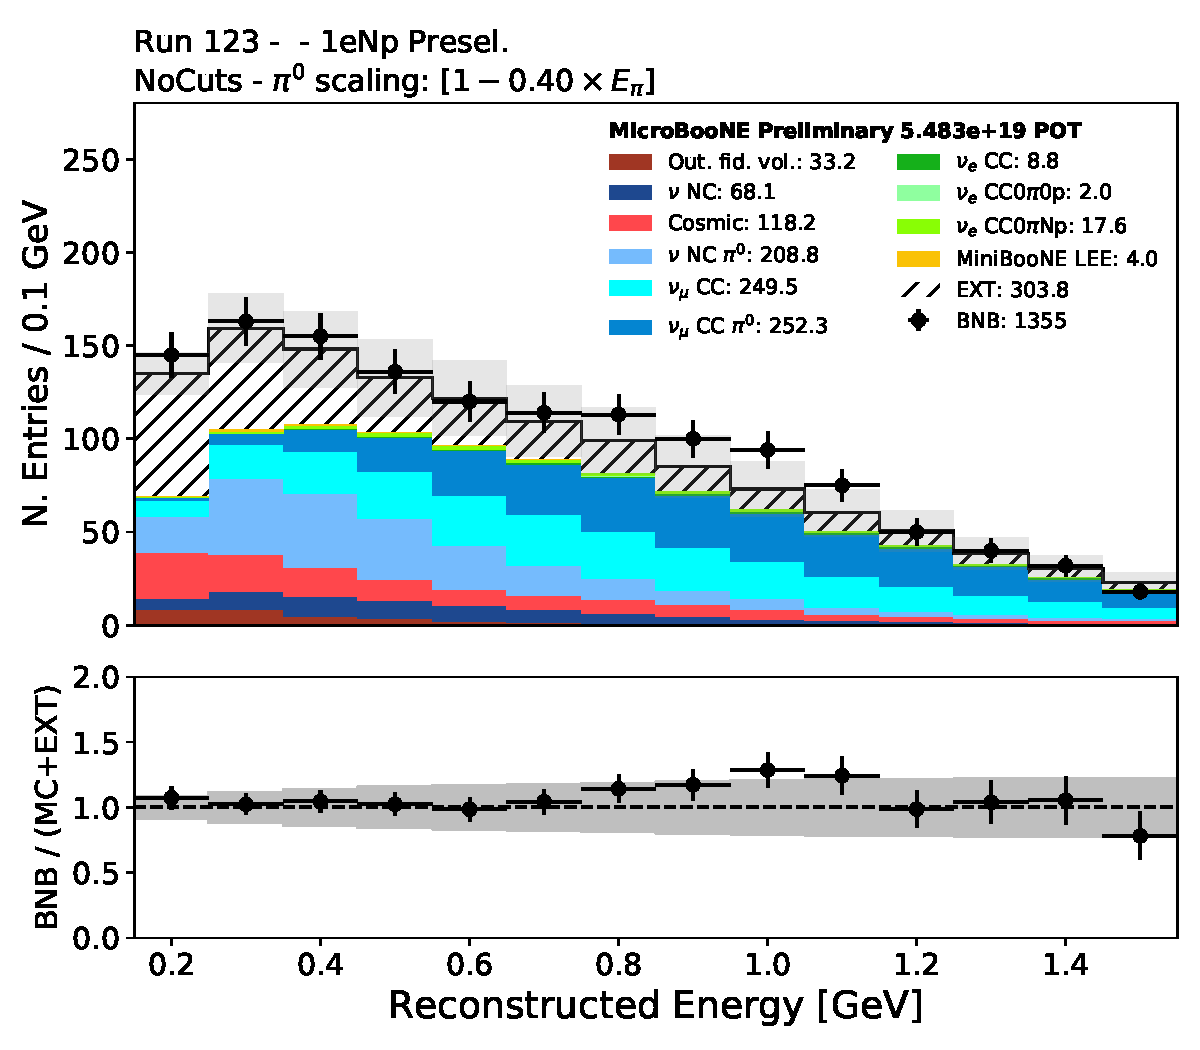
\includegraphics[width=0.6\textwidth]{1eNp/reco_e_presel.pdf}
\caption{\label{fig:1eNp:prsel}Reconstructed neutrino energy after pre-selection for the \npsel channel.}
\end{center}
\end{figure}

%\begin{figure}[ht] 
%\begin{center}
%    \begin{subfigure}[b]{0.45\textwidth}
%    \centering
%    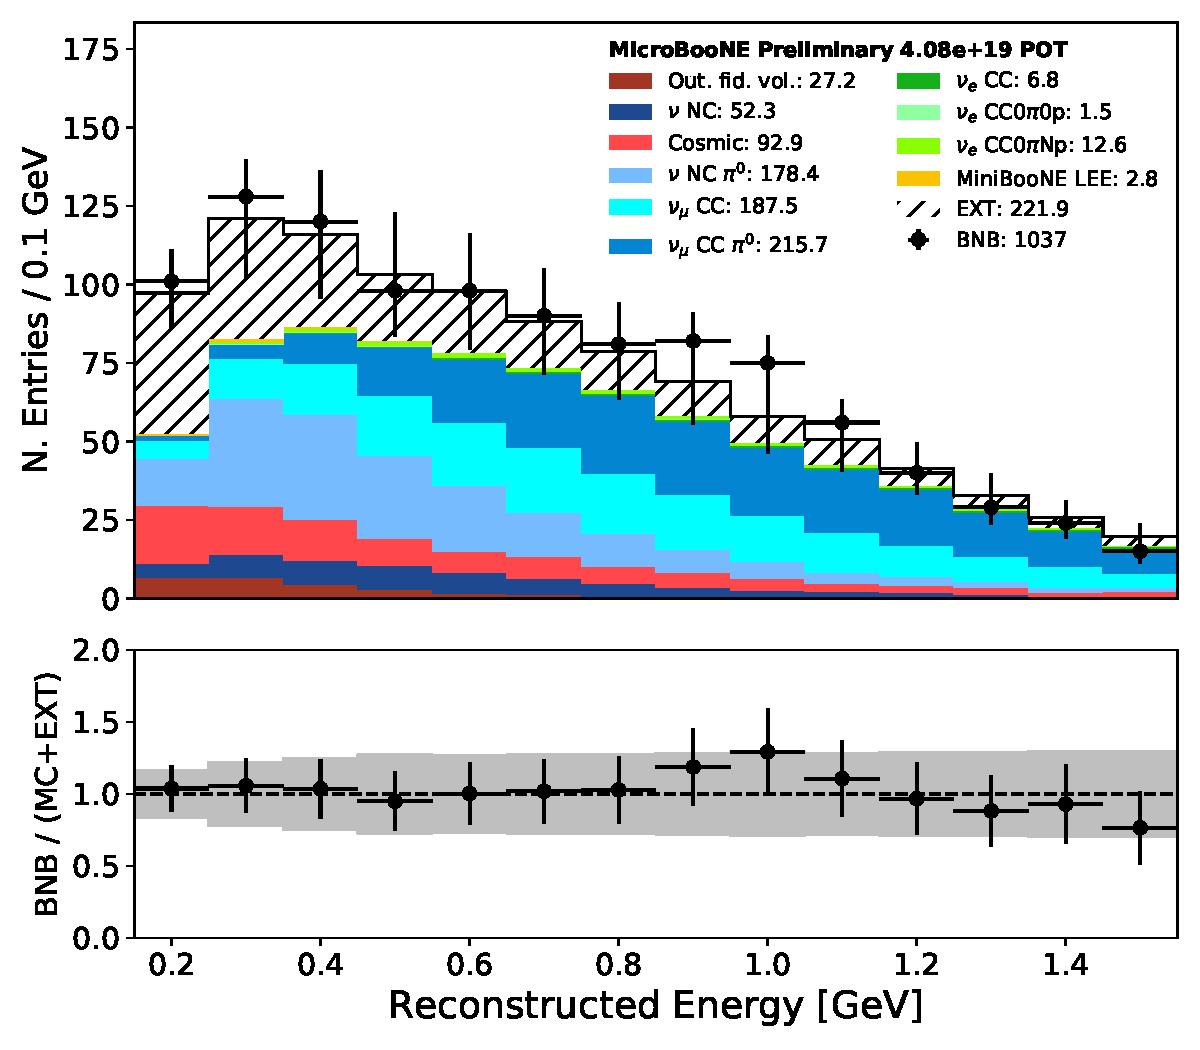
\includegraphics[width=1.00\textwidth]{1eNp/reco_e_03122020_RUN1_preselection.pdf}
%    \caption{\label{fig:1eNp:prsel:RUN1} RUN 1}
%    \end{subfigure}
%    \begin{subfigure}[b]{0.45\textwidth}
%    \centering
%    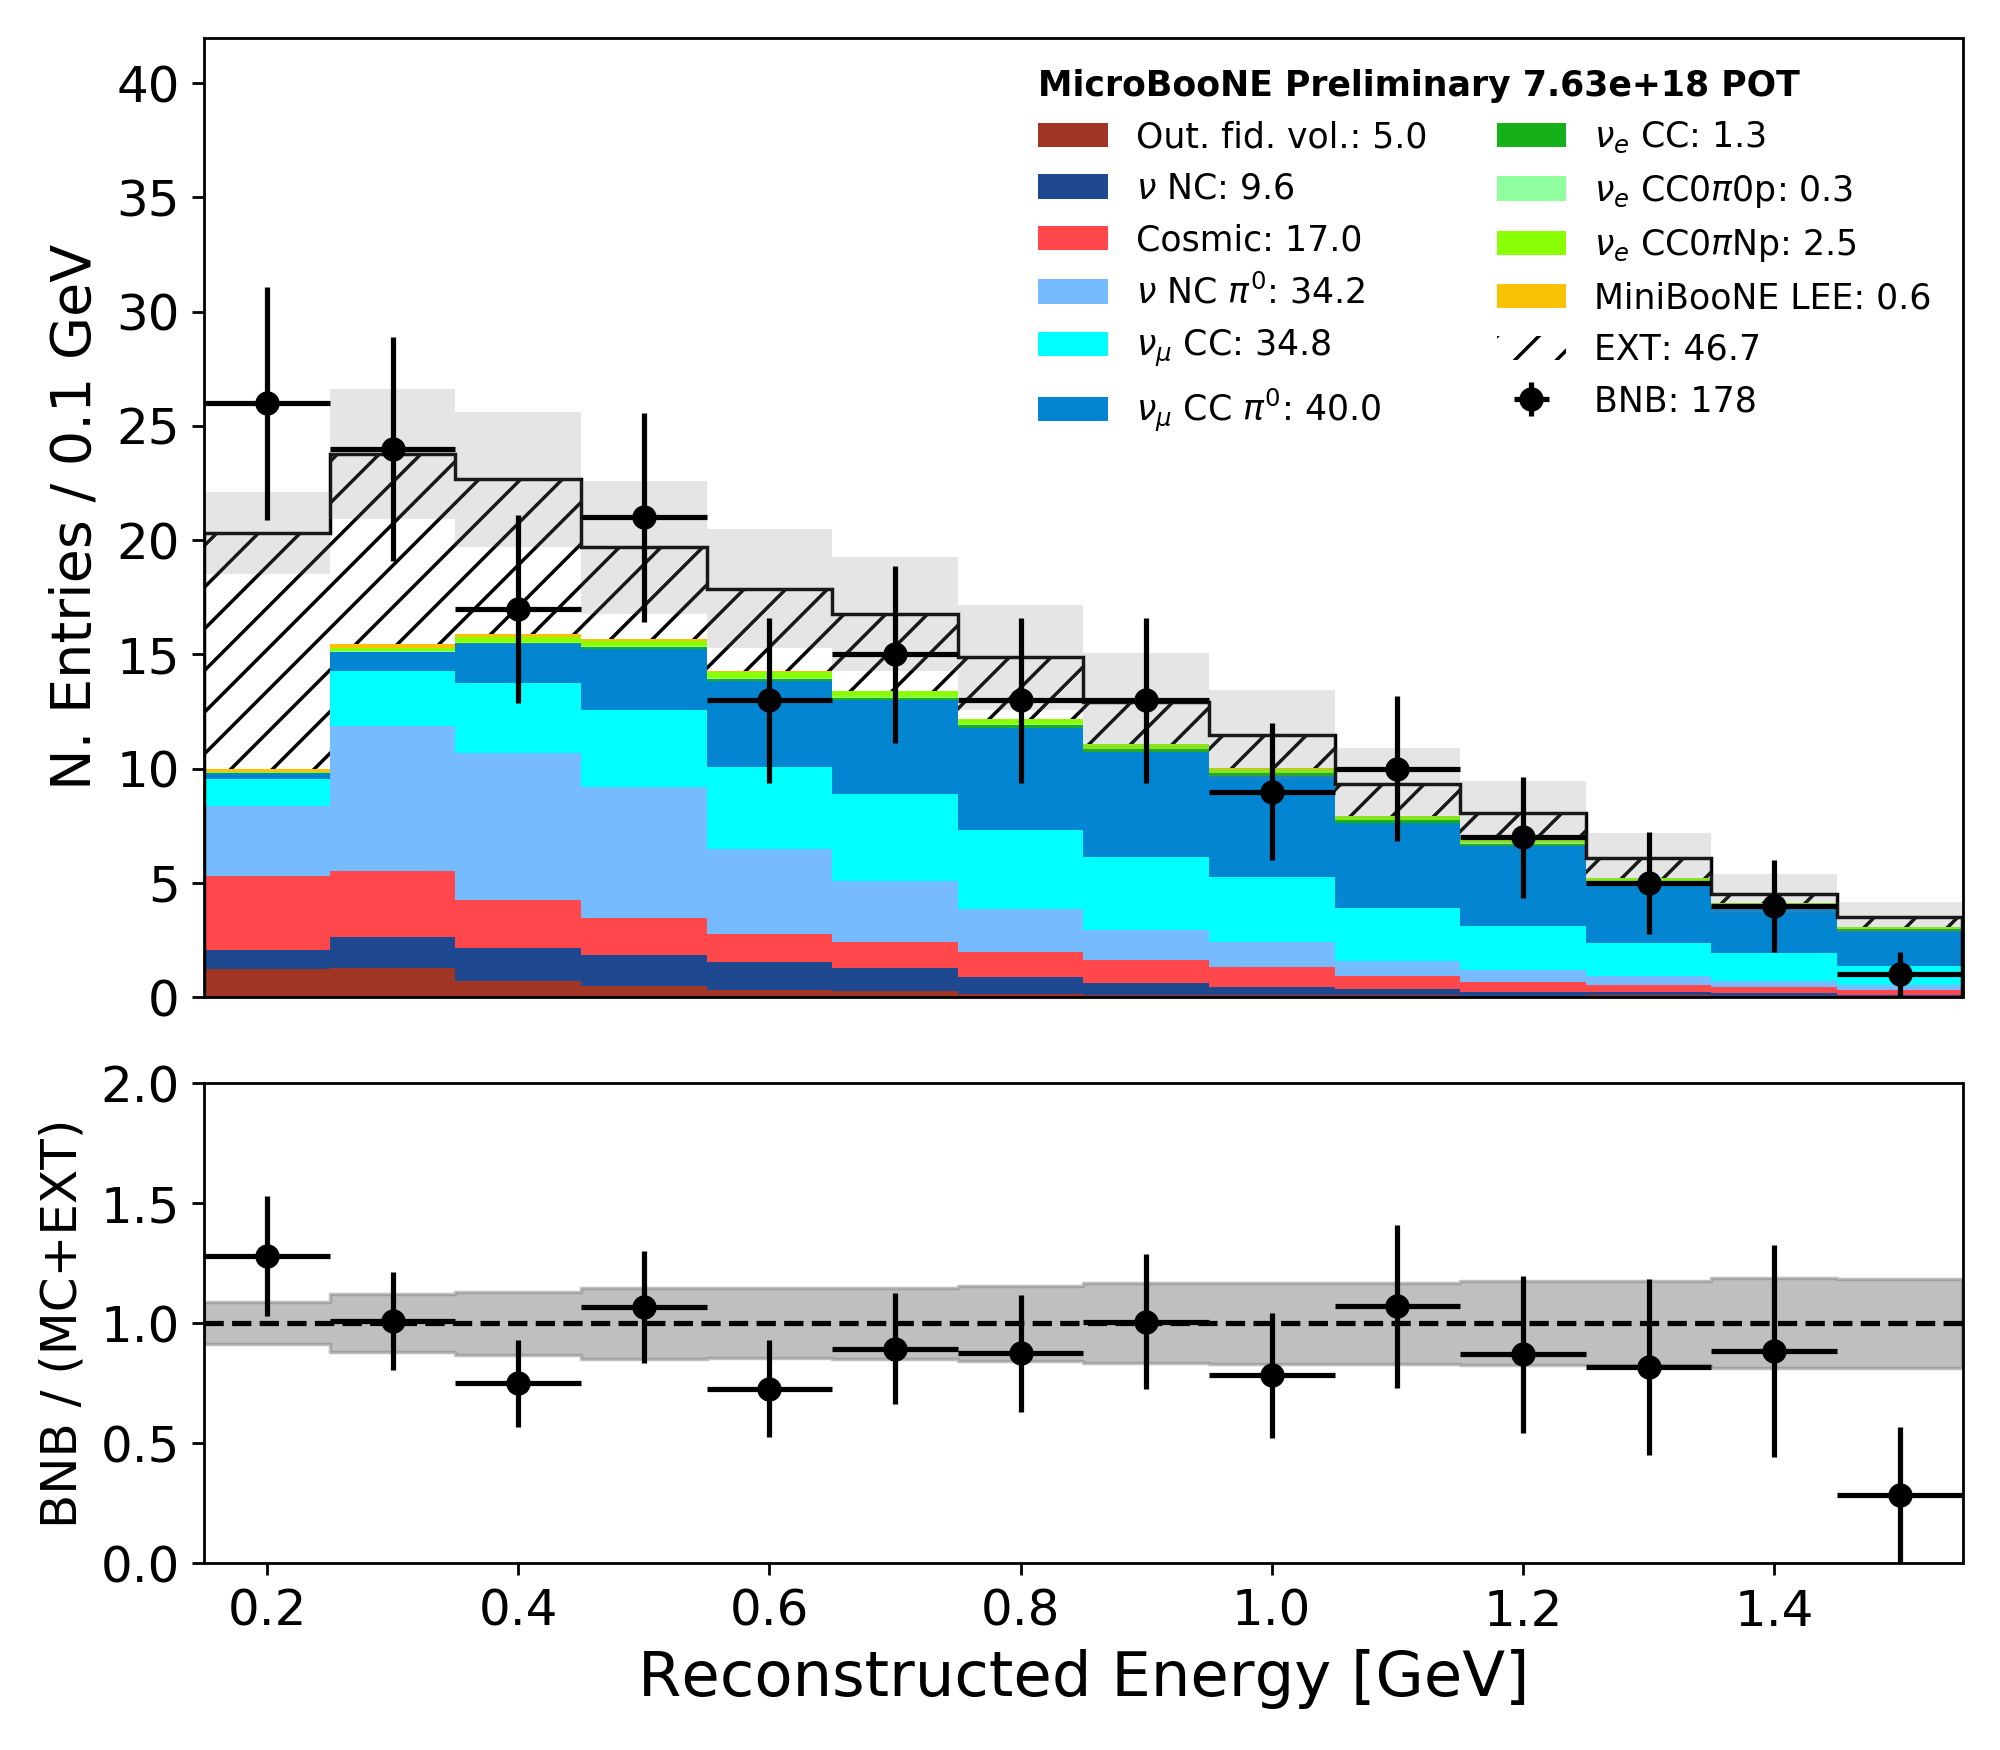
\includegraphics[width=1.00\textwidth]{1eNp/reco_e_03122020_RUN3_preselection_fixed.png}
%    \caption{\label{fig:1eNp:prsel:RUN1} RUN 3}
%    \end{subfigure}
%\caption{\label{fig:1eNp:prsel}Reconstructed neutrino energy after pre-selection for the \npsel channel.}
%\end{center}
%\end{figure}


\subsubsection{\npsel Selection}

Both a box-cut and BDT-based selection have been developed for the \npsel. The BDT-based selection is expected to be the most sensitive to low-energy \nue events since BDTs are able to learn additional information from the data and return a response variable that is highly discriminating between signal and background. The box-cut selection, relying on the same input variables, can provide a robust validation of the analysis, though with lower signal sensitivity. It is documented in Appendix~\ref{app:nueslections:1eNp}. In the remainder of this section we present exclusively the BDT-based selection.

Two BDTs are trained separately to reject backgrounds with and without $\pi^0$ in the final state. The same set of training variables is used in the two BDTs, corresponding to the list of variables used in the box-cut selection. In order to avoid splitting the already limited-size samples used for the analysis, dedicated samples are used for training: the signal comes from intrinsic \nue samples in the range $0<E_\nu<400$ and $0<E_\nu<800$ \si{GeV}; EXT events are taken from a sample of about 280k events from the NuMI EXT data stream; $\pi^0$ samples for BDT training are produced recycling the EXT unbiased events used in the overlay procedure; non-$\pi^0$ neutrino-induced background samples are produced with tight filters on truth-variables that enhance $\nu_{\mu}$ 0$\pi^0$ events that contribute as backgrounds to the analysis. (\href{https://microboone-docdb.fnal.gov/cgi-bin/private/RetrieveFile?docid=28140&filename=tight-nue-back-filter-merge-memo.pdf&version=1}{DocDB 28140}). As a result the relative size of the samples varies significantly, so the event weight in training is enhanced for specific categories of backgrounds such as \numucc events with no pions or EXT and cosmic-dominated events. Training is performed after requiring \texttt{reco\_e $<$ 0.8} and \texttt{n\_showers\_contained $=$ 1} on top of the \npsel pre-selection.  

The BDT training is able to figure out which variables are most important for each background. Figure~\ref{ffig:1eNp:bdt:var} shows that, while the importance of the training variable is in general very similar in the two BDTs, there are indications that each BDT specializes for their target background; for instance, the most discriminating variable is different, being subcluster for the non-$\pi^0$ BDT and tksh\_distance for the $\pi^0$ BDT. %It is interesting to note that the most discriminating variable in both cases is shrmoliereavg, since it can be useful to discriminate both muons in $\nu_\mu$ events (low values) and merged showers in $\pi^0$ events (large values).
Validations of the BDT training variables in terms of data-MC comparison on the unbiased Run1 + Run3 5e19 datasets are presented in appendix~\ref{app:nuepresel}. Further validations of data/MC agreement from low-PID, 2+ shower, and high-energy $\nu_e$ sidebands are included in Sec.~\ref{sec:sideband:1eNp:lowpid},~\ref{sec:sideband:1eNp:2pshr}, and~\ref{sec:sideband:1eNp:he} respectively.

\begin{figure}[H] 
\begin{center}
    \begin{subfigure}[b]{0.45\textwidth}
    \centering
    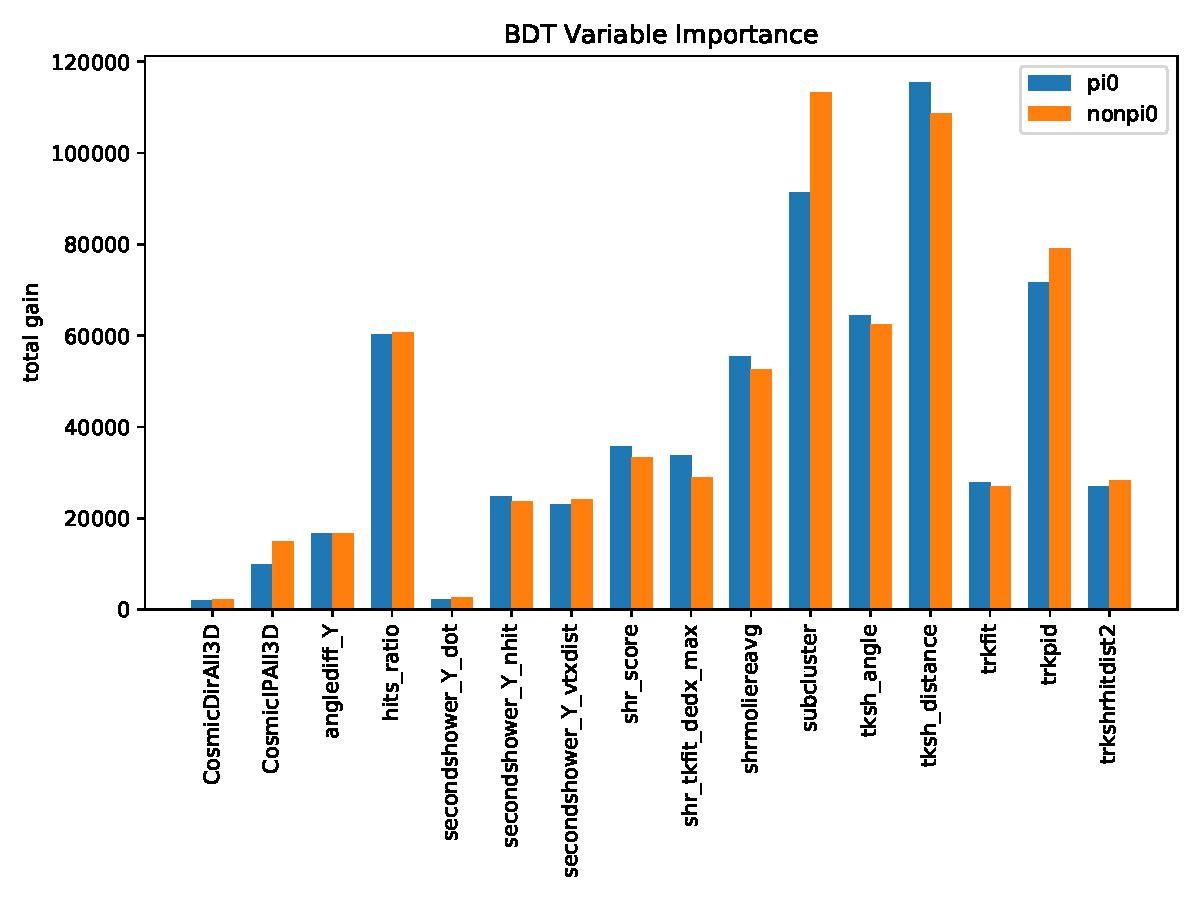
\includegraphics[width=1.00\textwidth]{1eNp/bdt_var_gain.pdf}
    \caption{\label{fig:1eNp:bdt:var:gain}}
    \end{subfigure}
    \begin{subfigure}[b]{0.45\textwidth}
    \centering
    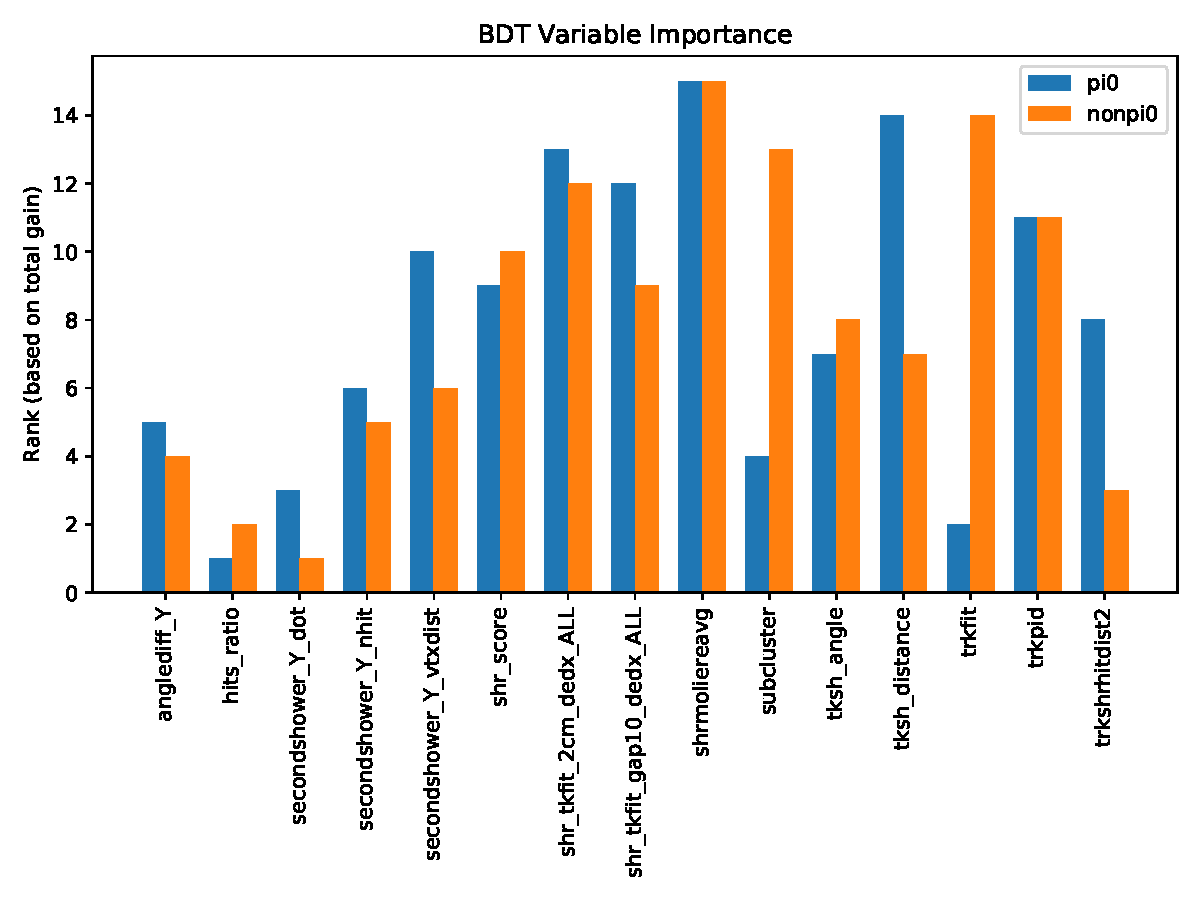
\includegraphics[width=1.00\textwidth]{1eNp/bdt_var_rank.pdf}
    \caption{\label{fig:1eNp:bdt:var:rank}}
    \end{subfigure}
\caption{\label{ffig:1eNp:bdt:var} BDT variables importance in terms of ``total gain". In \texttt{xgboost}~\cite{bib:xgboost}, "gain" is the improvement in accuracy brought by a feature to the branches it is on; "total gain" refers to the sum of the "gain" across all branches. Left: total gain value. Right: ranking based on the total gain value (highest ranking=15, lowest=1).}
\end{center}
\end{figure}

The BDT selection combines a set of loose box cuts and cuts on BDT responses. The loose box cuts are listed in Table~\ref{tab:1eNp:loosecut} and are intended to reject events where one or more variables are clearly inconsistent with \nuecc interactions. The resulting BDT responses in Run1 open data are shown in Figures~\ref{fig:1eNp:bdt:nonpi0} and \ref{fig:1eNp:bdt:pi0} for the non-$\pi^0$ and $\pi^0$ BDT, respectively. The left and right panels show the response below and above 0.5 respectively. We cut separately on the output of the two BDTs, requiring the $\pi^0$ and non-$\pi^0$ responses to be greater than 0.67 and 0.70, respectively. The cut flow table in terms of efficiency and purity at low energy is in Fig. \ref{fig:1eNp:cutflow:bdt}. The resulting reconstructed \nue energy after the BDT selection is shown in Figure~\ref{fig:1eNp:bdt:1e21}. %The (purity, efficiency) change from (0.6\%,33\%) $\righarrow$ (12\%, 12\%) $\rightarrow$ (65\%, 9\%) at pre-selection, loose box-cut, and BDT cut, respectively. The final BDT cut allows for a more than 4$\times$ increase in purity with a relative efficiency of 75\%.

Two events pass the full BDT selection in the available $4.07E19$ POT dataset from Run1. Both events appear to be good $\nu_e$ candidates (consistent with the level of purity expected), and are reconstructed with $\sim 1.1$ GeV of energy; event displays are shown in Fig.~\ref{fig:1eNp:box:evd}.

%\emph{The BDT selection can be considered final, pending more detailed checks of data-MC agreement with large statistics and the availability of additional samples for training.}

\begin{table}[h!]
\centering
\setlength{\tabcolsep}{10pt}
\renewcommand{\arraystretch}{1.25}
 \begin{tabular}{| c | c |} 
 \hline
 Cut goal & Cut definition \\
 \hline\hline
\multirow{2}{*}{Cosmic~rejection} & CosmicIPAll3D $>$ 10 \si{\cm} \\
& trkpid $<$ 0.02 \\
 \hline
\multirow{5}{*}{$\nu_\mu$~rejection} & hits\_ratio $>$ 0.5 \\
& shrmoliereavg $<$ 9\si{\degree} \\
& subcluster $>$ 4 \\
& trkfit $<$ 0.65 \\
& shr\_trk\_len $<$ 300 cm \\
 \hline
\multirow{3}{*}{$\pi^0$~rejection} & n\_showers\_contained = 1 \\
& tksh\_distance $<$ 6.0 \si{\cm} \\
& shr\_tkfit\_nhits\_tot $>$ 1 and 0.5 $<$ shr\_tkfit\_dedx\_max $<$ 5.5 \si{\MeV}/\si{\cm} \\
%& secondshower\_Y\_nhit $<$ 50 \\
 \hline
Misreconstruction & tksh\_angle $>$ -0.9 \\
 \hline
 \end{tabular}
 \caption{\label{tab:1eNp:loosecut} Loose cut requirements for the \npsel BDT selection.}
\end{table}

\begin{figure}[H] 
\begin{center}
    \begin{subfigure}[b]{0.45\textwidth}
    \centering
    % p-values: nonpi0_score 0.2647 0.9388 0.8853
    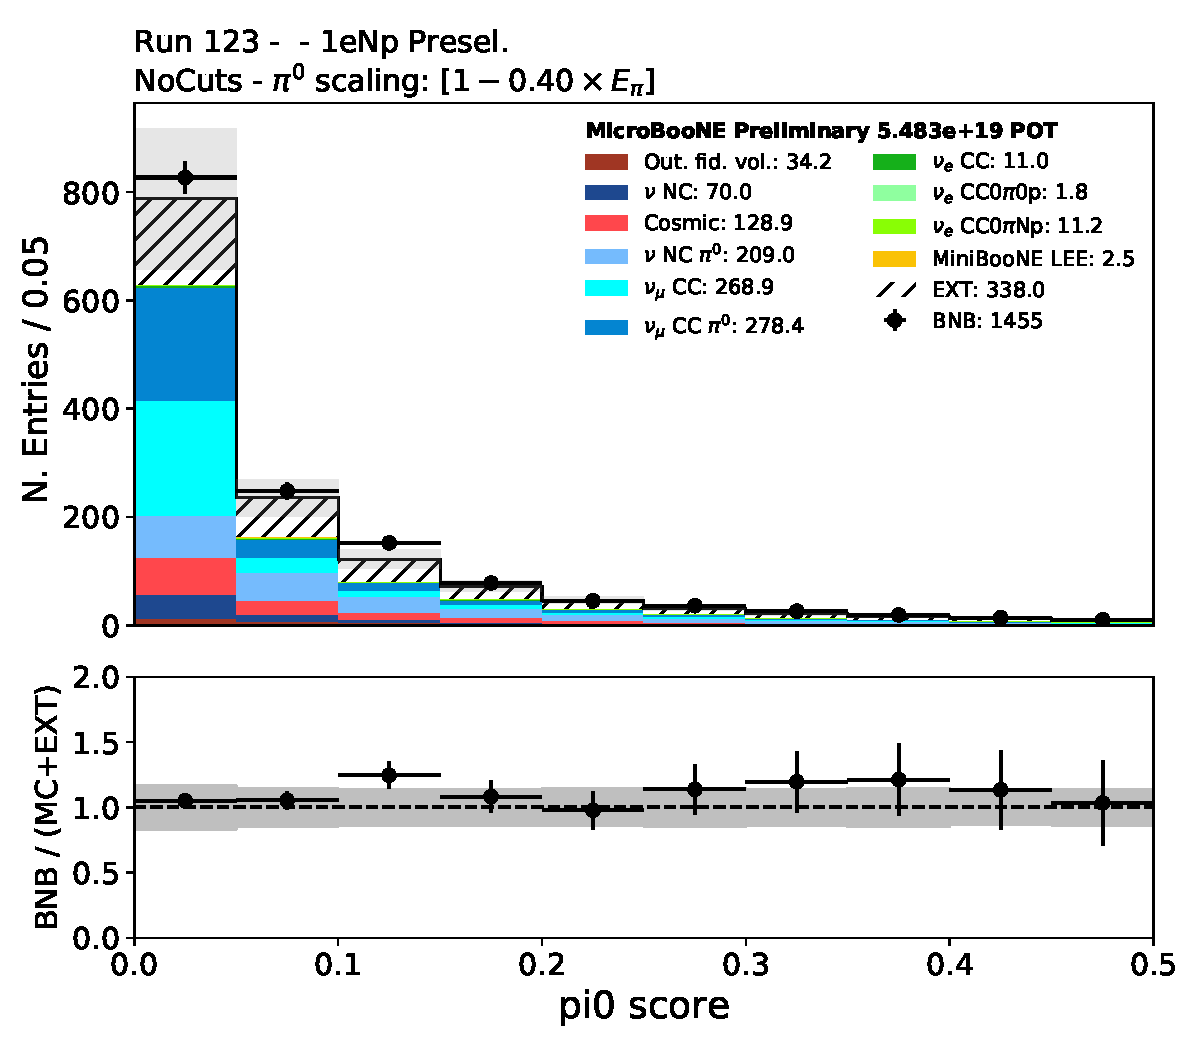
\includegraphics[width=1.00\textwidth]{1eNp/nonpi0_score_presel_low.pdf}
    \caption{\label{fig:1eNp:bdt:nonpi0:low}}
    \end{subfigure}
    \begin{subfigure}[b]{0.45\textwidth}
    \centering
    % p-values: nonpi0_score 0.0288 0.0554 0.0671
    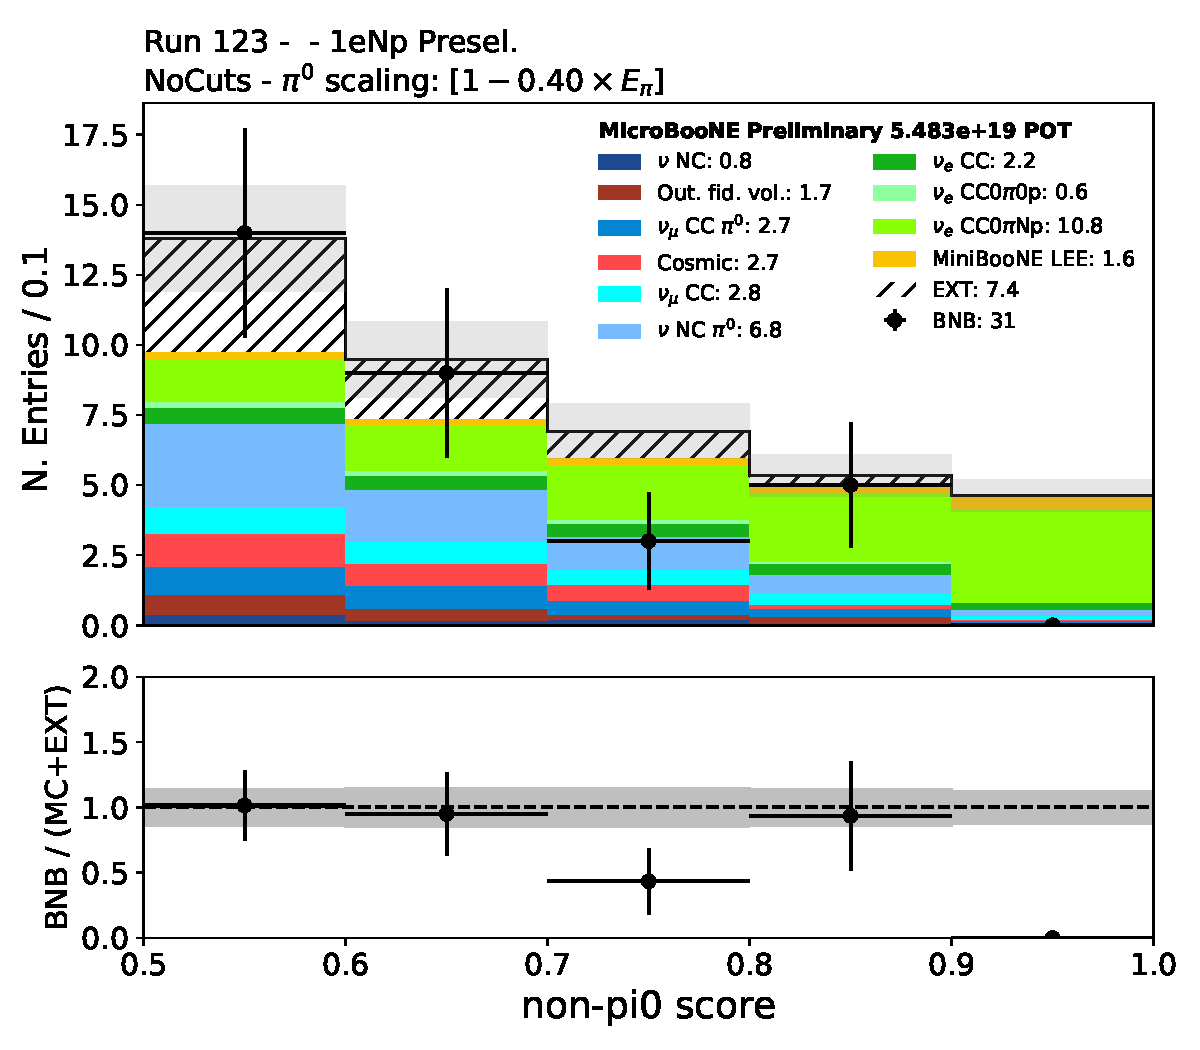
\includegraphics[width=1.00\textwidth]{1eNp/nonpi0_score_presel_high.pdf}
    \caption{\label{fig:1eNp:bdt:nonpi0:high}}
    \end{subfigure}
\caption{\label{fig:1eNp:bdt:nonpi0}BDT response for non-$\pi^0$ BDT after \npsel pre-selection}
\end{center}
\end{figure}

\begin{figure}[H] 
\begin{center}
    \begin{subfigure}[b]{0.45\textwidth}
    \centering
    % p-values: pi0_score 0.1076 0.6487 0.5926
    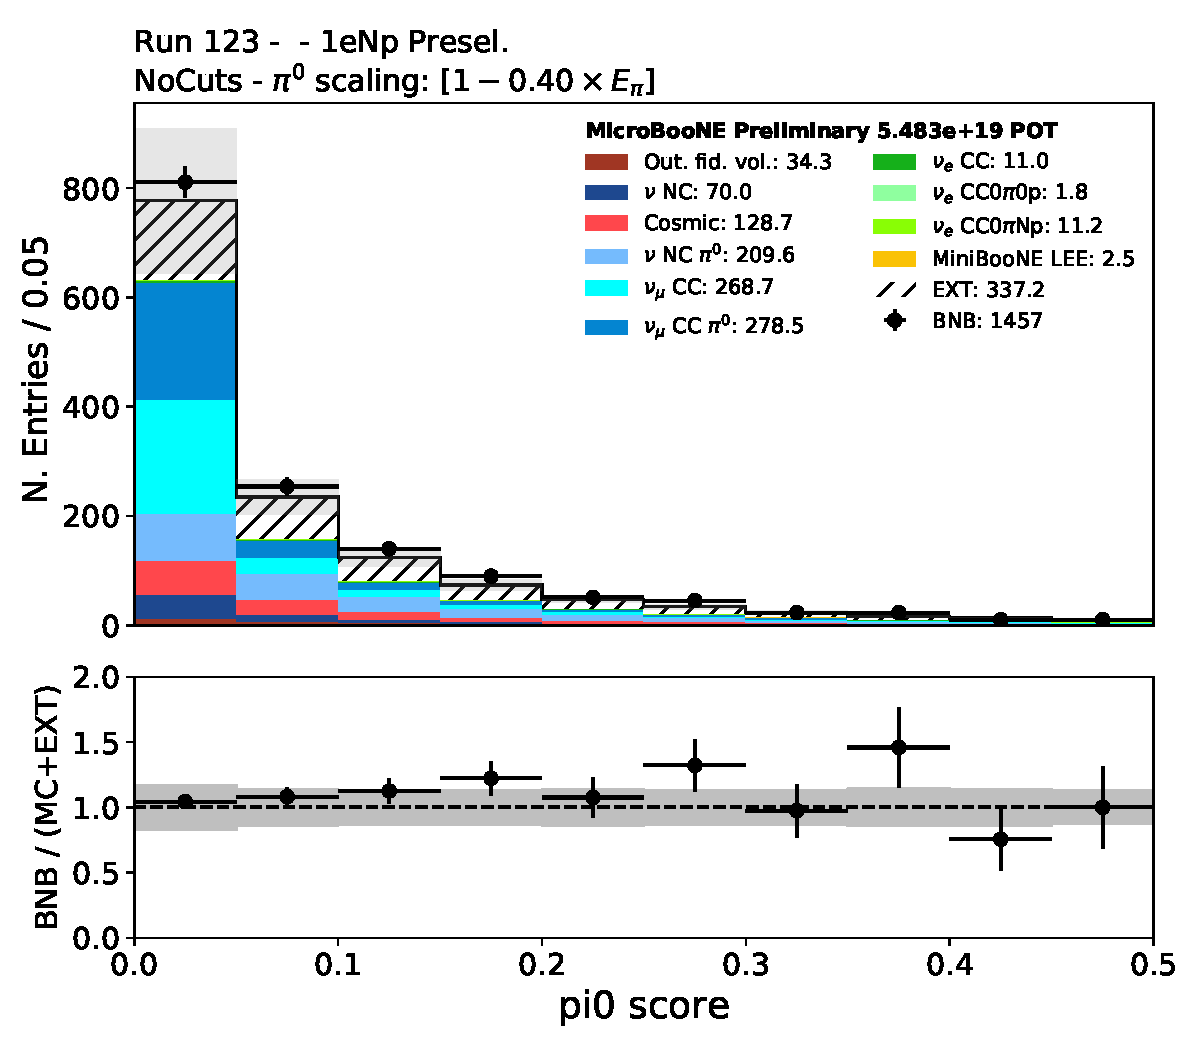
\includegraphics[width=1.00\textwidth]{1eNp/pi0_score_presel_low.pdf}
    \caption{\label{fig:1eNp:bdt:pi0:low}}
    \end{subfigure}
    \begin{subfigure}[b]{0.45\textwidth}
    \centering
    % p-values: pi0_score 0.1012 0.1609 0.2412
    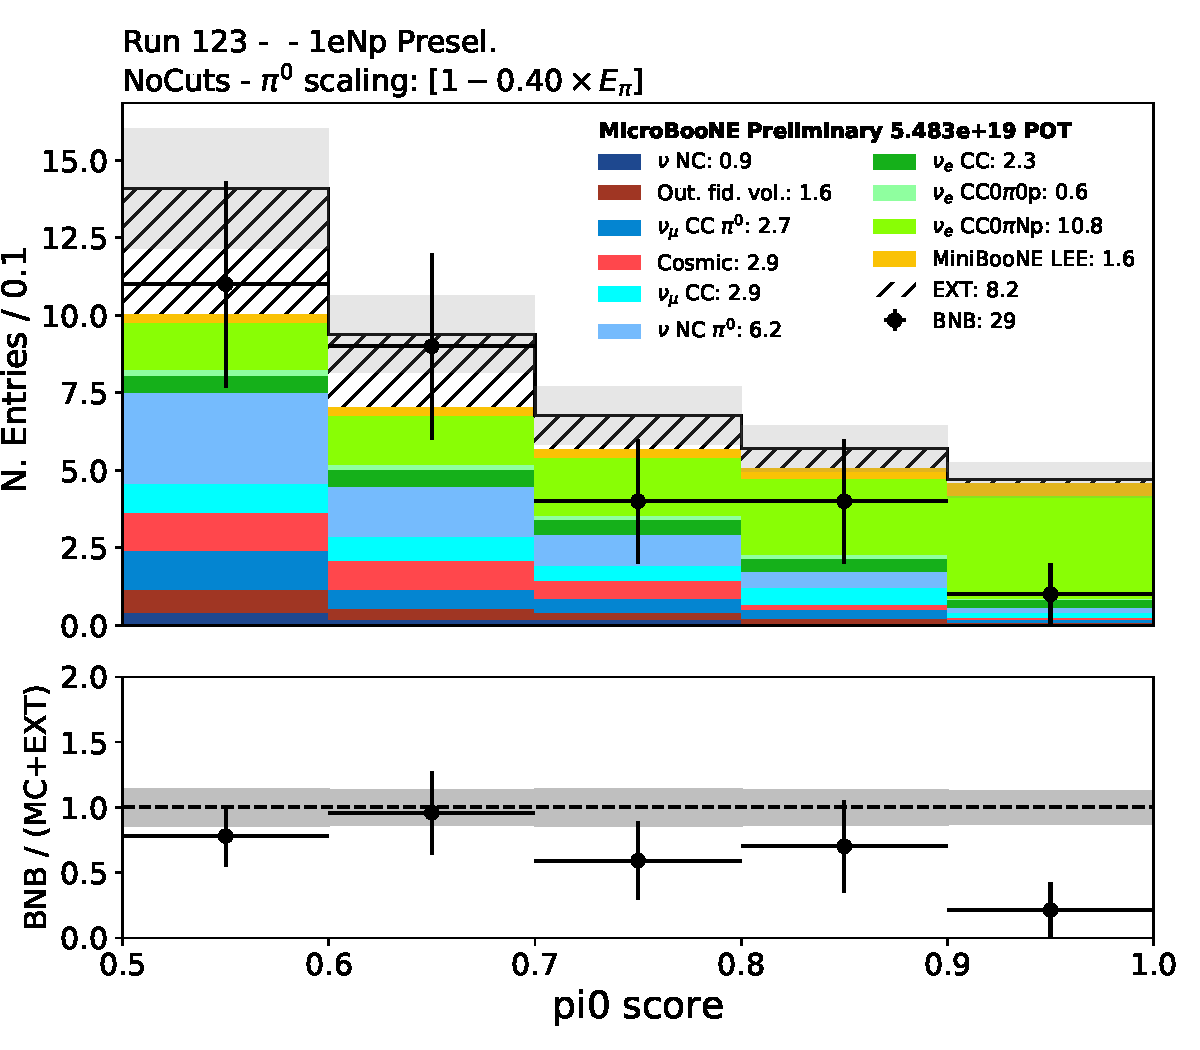
\includegraphics[width=1.00\textwidth]{1eNp/pi0_score_presel_high.pdf}
    \caption{\label{fig:1eNp:bdt:pi0:high}}
    \end{subfigure}
\caption{\label{fig:1eNp:bdt:pi0}BDT response for $\pi^0$ BDT after \npsel pre-selection}
\end{center}
\end{figure}

\begin{figure}[H]
\begin{center}
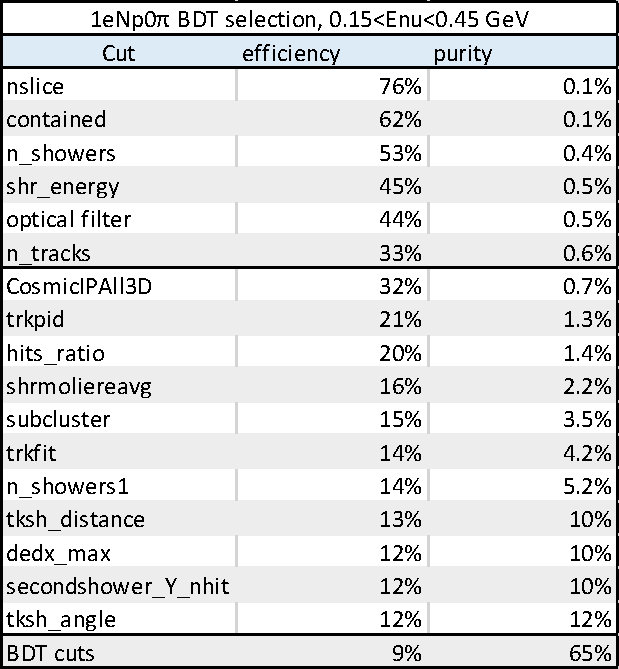
\includegraphics[width=0.40\textwidth]{1eNp/cuts-eff-pur-bdt.pdf}
\caption{\label{fig:1eNp:cutflow:bdt} Efficiency and purity for cuts in the BDT \npsel selection. Values are cumulative and are computed for neutrino energy between 0.15 and 0.45 GeV. }
\end{center}
\end{figure}

\begin{figure}[H]
\begin{center}
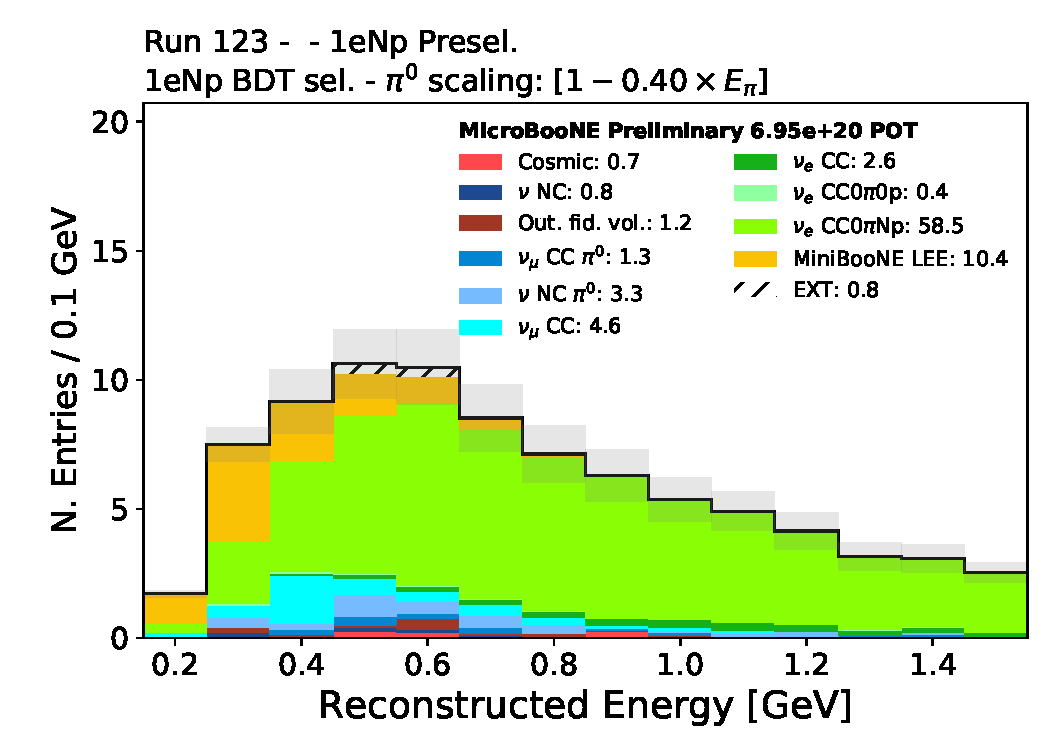
\includegraphics[width=0.65\textwidth]{1eNp/reco_e_BDT.pdf}
\caption{\label{fig:1eNp:bdt:1e21}BDT-based selection for \npsel with cuts at 0.67 and 0.70 for the $\pi^0$ and non-$\pi^0$ variables respectively.}
\end{center}
\end{figure}

\begin{figure}[H] 
\begin{center}
    \begin{subfigure}[b]{0.45\textwidth}
    \centering
    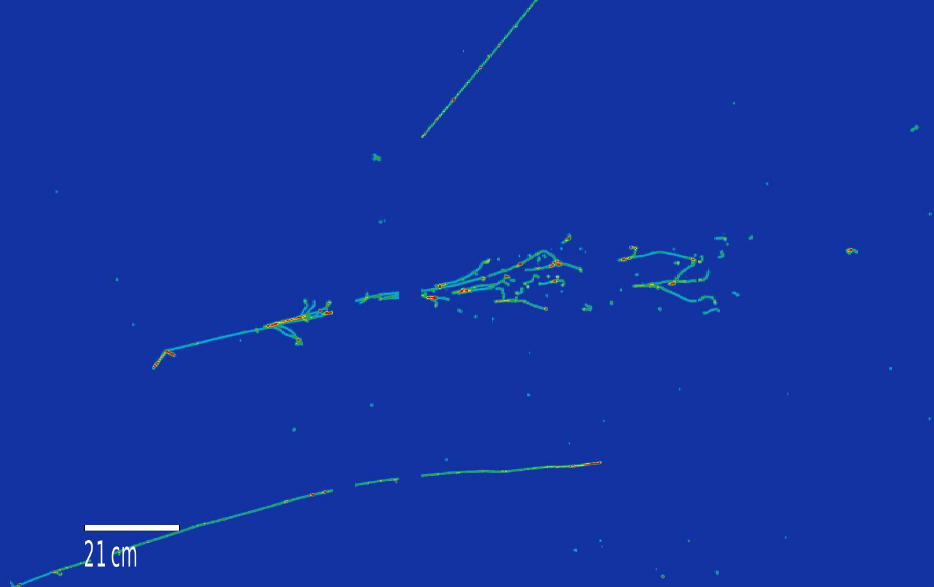
\includegraphics[width=1.00\textwidth]{1eNp/1eNp_box_evd1.png}
    \caption{\label{fig:1eNp:box:evd1}1.10 GeV [reco] $\nu_e$ candidate}
    \end{subfigure}
    \begin{subfigure}[b]{0.45\textwidth}
    \centering
    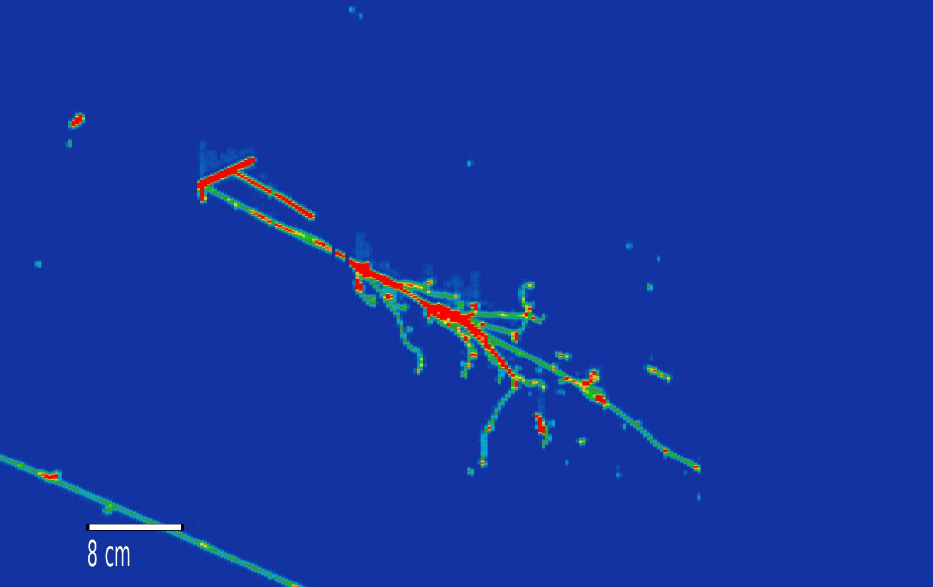
\includegraphics[width=1.00\textwidth]{1eNp/1eNp_box_evd2.png}
    \caption{\label{fig:1eNp:box:evd2}1.07 GeV [reco] $\nu_e$ candidate}
    \end{subfigure}
\caption{\label{fig:1eNp:box:evd} \npsel candidates from the open $4E19$ Run1 open dataset. After the \npsel preselection, two data events with BDT score $> 0.8$ are found.}
\end{center}
\end{figure}

\subsubsection{Performance of \npsel selections}

Figure~\ref{fig:1eNp:effpur:RUN3} shows the efficiency and purity of the \npsel selections as a function of the neutrino energy. The efficiency is already low at preselection level, especially for neutrino energies below 0.8 \si{\GeV}. This demonstrates how challenging it is to properly identify and reconstruct such events. The loose cuts then are able to improve the purity by about one order of magnitude at the price of a 2-3x reduction in efficiency. The BDT and box cut selections then further improve the purity by up to a factor 7, with a reduction in efficiency of $\sim$25\% ($\sim$50\%) for the BDT (box cut) selections . With the full Run 1+2+3 dataset of  6.95e20 POT dataset, the expected number of MiniBooNE LEE signal events identified with the BDT selection is about 10.4, and the expected number of intrinsic $\nu_e$ events is 62.5.

\begin{figure}[H]
\begin{center}
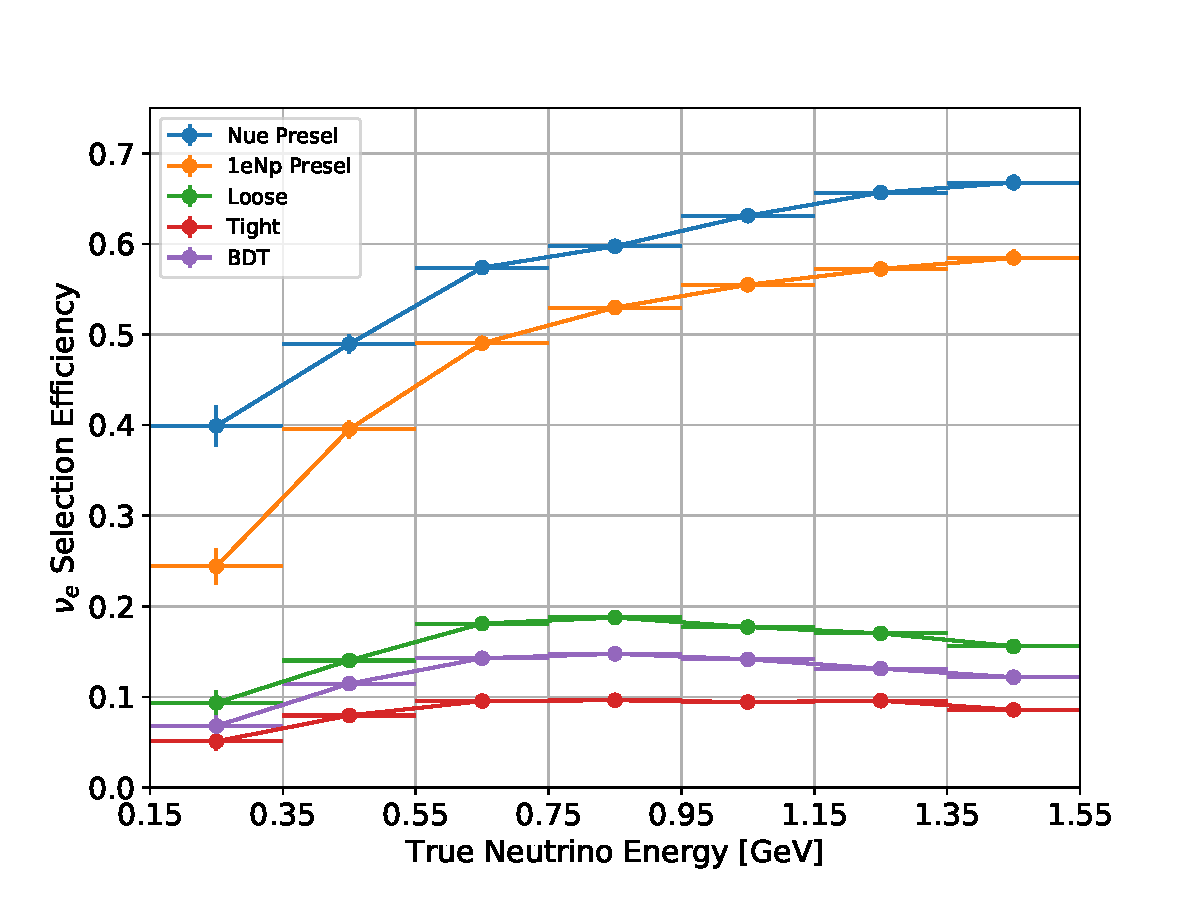
\includegraphics[width=0.45\textwidth]{1eNp/eff_1eNp_cut_bdt.pdf}
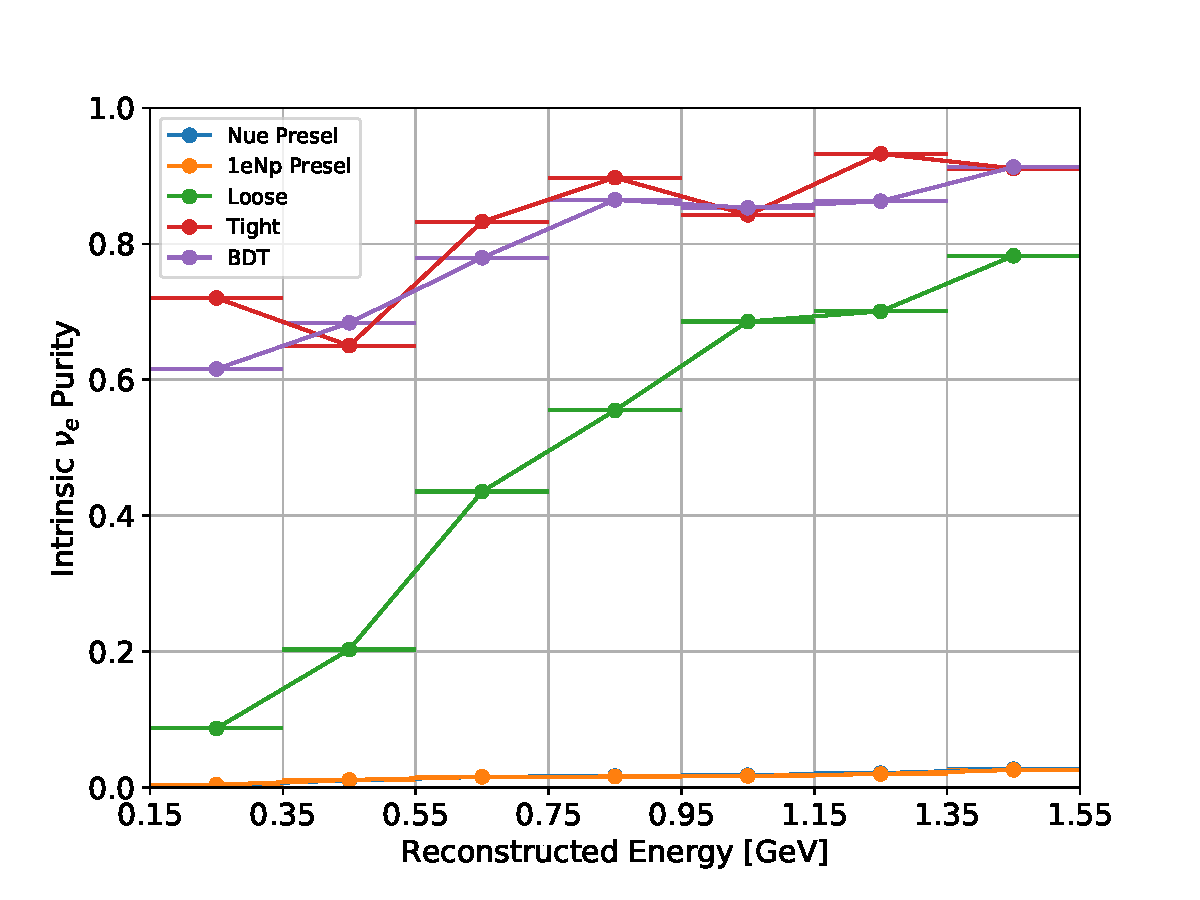
\includegraphics[width=0.45\textwidth]{1eNp/pur_1eNp_cut_bdt.pdf}
\caption{\label{fig:1eNp:effpur:RUN3} Efficiency (left) and purity (right) of different selections for true contained \npsel events. The purity refers to the intrinsic \npsel only (a possible MiniBooNE LEE signal is not considered).}
\end{center}
\end{figure}

The final signal efficiency turns out to be rather low, in the 5-15\% range for the box cut and BDT selections. A large efficiency loss is introduced already at pre-selection level, which consists of very basic requirements that are mostly needed to define the other selection variables. As already discussed, the BDT selection greatly enhances the purity but this comes at a price of a further efficiency loss. The absolute efficiency of each of the cuts as defined in the box-cut selection~\ref{app:nueslections:1eNp} on top of the pre-selection is shown in Fig.~\ref{fig:1eNp:abseff:RUN3} and \cref{fig:1eNp:cutflow:rel}. No single cut has an efficiency lower than 50\%. To isolate the cause of the selection inefficiency, we compute the efficiency for the subset of events where the shower start is reconstructed within one cm of the true vertex position (fig.~\ref{fig:1eNp:abseff:RUN3}, right) and find a significant improvement in performance, pointing to vertex reconstruction as one fo the main limitations in the reconstruction. In summary, the two main reasons for the low efficiency of the analysis are the pre-selection requirements and the vertex position reconstruction accuracy. In order to increase the analysis' efficiency, work aimed at improving the underlying reconstruction is needed. This work is beyond the scope of the analysis currently developed. This fact does not take away that the level of performance achieved with current tools is able to produce valuable and interesting results.

\begin{figure}[H]
\begin{center}
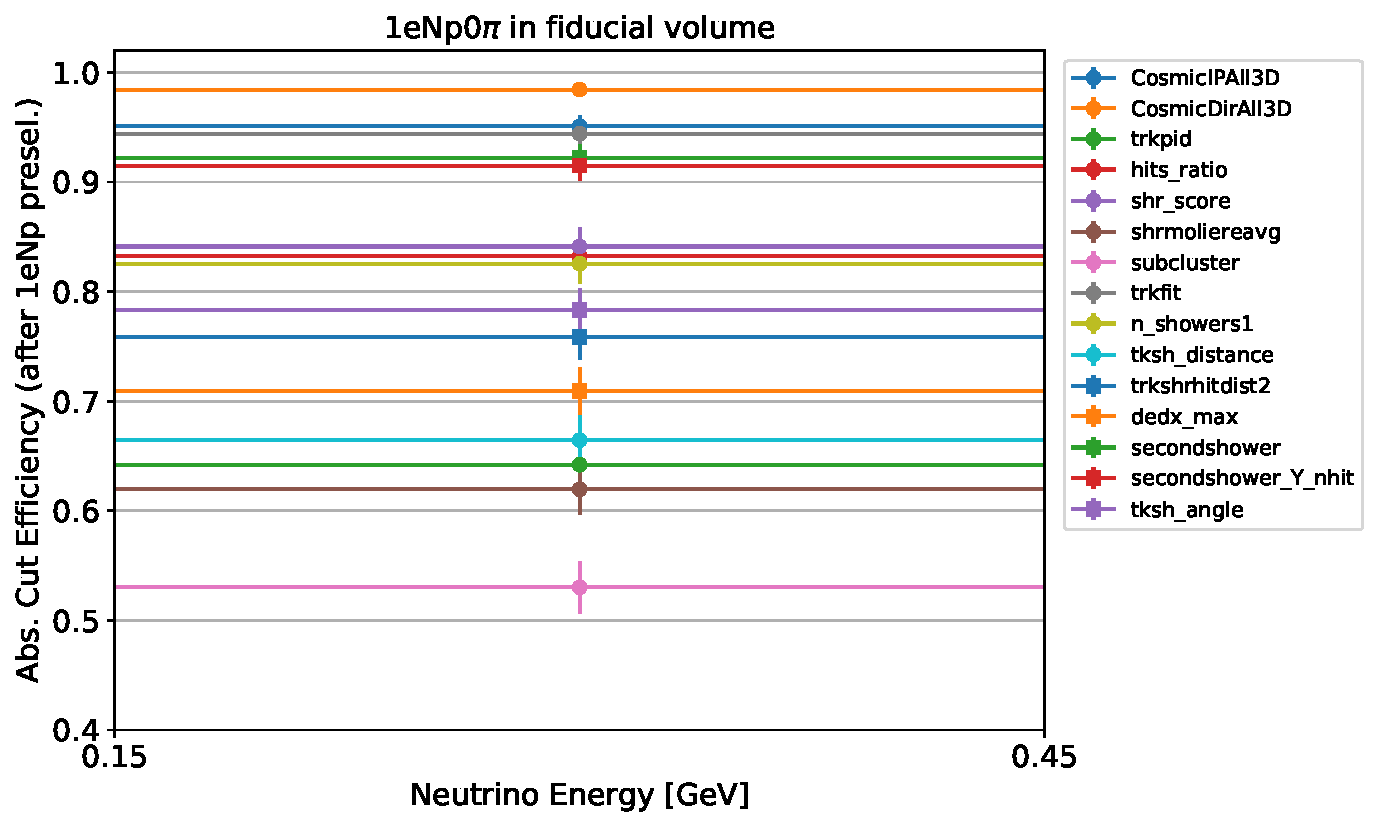
\includegraphics[width=0.45\textwidth]{1eNp/abseff_1eNp_cut_postpresel.pdf}
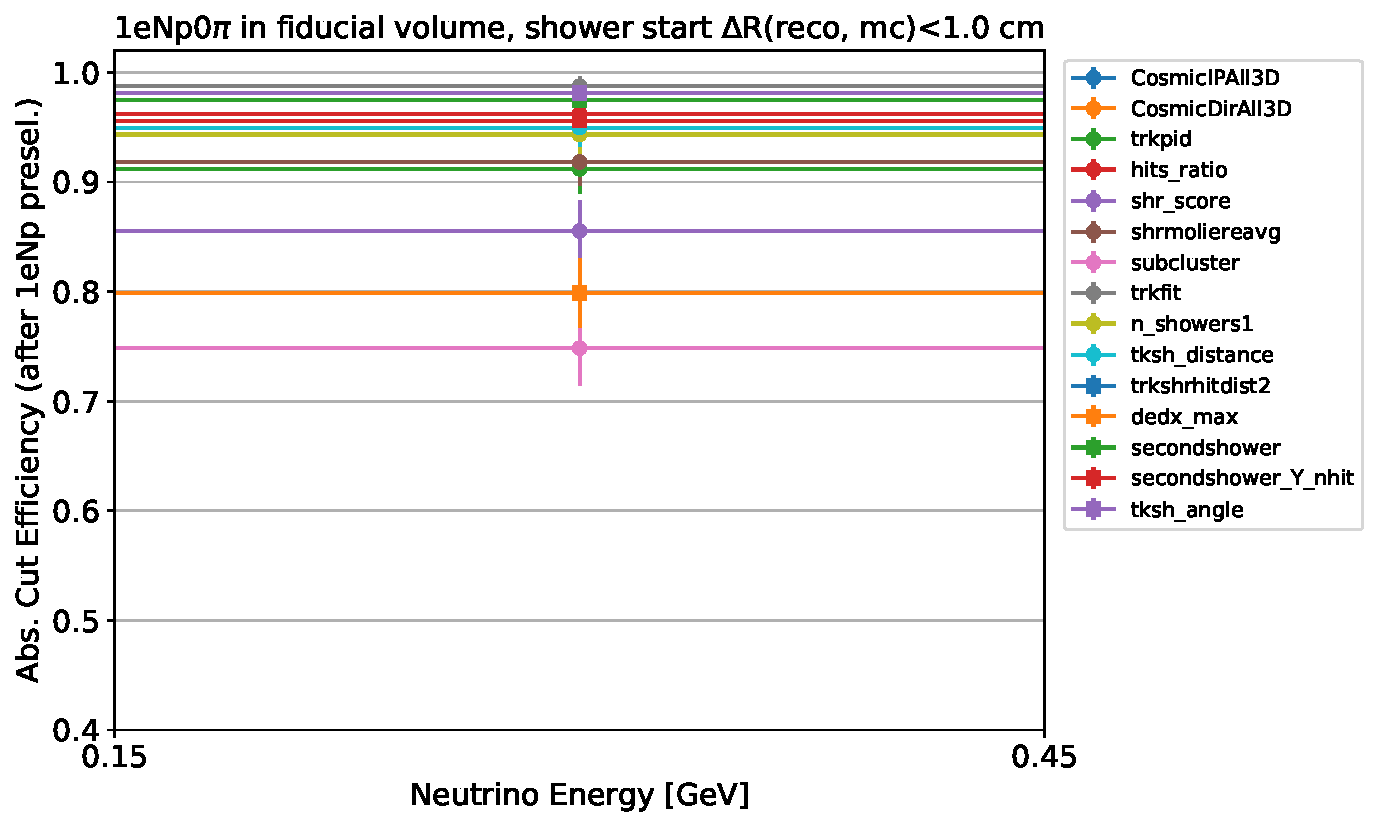
\includegraphics[width=0.45\textwidth]{1eNp/abseff_1eNp_cut_postpresel_drs.pdf}
\caption{\label{fig:1eNp:abseff:RUN3} Left: absolute efficiency of each of the box cuts on top of the pre-selection for \npsel events with $0.15<E_\nu<0.45~\si{GeV}$ that are in the fiducial volume. Right: same for the subset of events where the reconstructed shower start is within 1~\si{cm} of the true position. }
\end{center}
\end{figure}

\begin{figure}[H]
\begin{center}
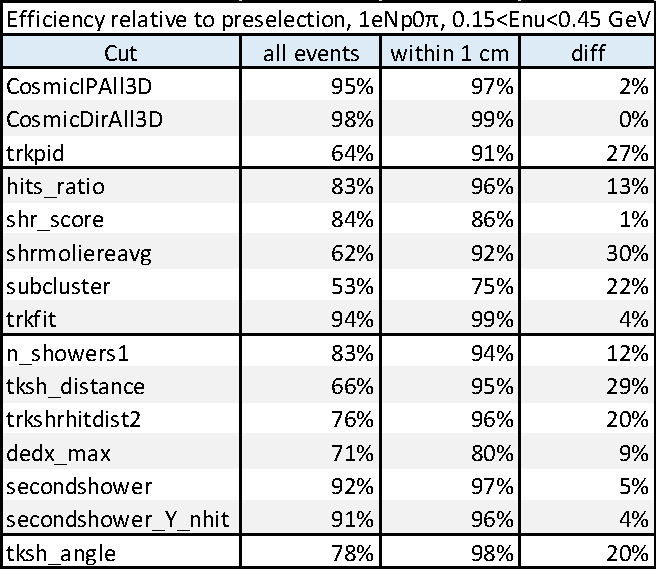
\includegraphics[width=0.40\textwidth]{1eNp/cuts-eff-rel-presel.pdf}
\caption{\label{fig:1eNp:cutflow:rel} Efficiency and purity for cuts in the tight box cut \npsel selection. Values are relative to pre-selection and are computed for neutrino energy between 0.15 and 0.45 GeV. Values are reported for all events, and for the subset with reconstructed vertex within 1 cm of the simulated one. The last column showes the difference. The content is the same as \cref{fig:1eNp:abseff:RUN3}. }
\end{center}
\end{figure}


\subsection{1$e$0$p$0$\pi$ Channel }
\label{sec:nueselection:1e0p}

The \zpsel topology complements the \npsel channel as it is a part of the signal that MiniBooNE measured. The MiniBooNE signal is defined as 1eXp0$\pi$, which is the sum of the \npsel and \zpsel channels. This means that including the \zpsel topology makes it possible for MicroBooNE to identify the full range of event topologies observed by MiniBooNE.    

The \zpsel channel can also be used to constrain uncertainties associated with the \npsel selection.  In particular, these are uncertainties associated with low energy protons, such as the modeling of the proton multiplicity and kinematics produced by neutrino interactions, as well as their reconstruction efficiencies.  This selection is particularly sensitive to the modeling of the hadronic component of the neutrino interaction, which makes it a useful way to constrain these systematics with data. An explicit example of why targeting such a channel is important comes from the observation that the version of Genie used in MCC8 predicted twice as many events in this channel as are expected in MCC9.  Also, in MCC8, half of the electron neutrinos below 0.8 GeV were in this channel, which is no longer the case in MCC9.

Since the \zpsel selection that will be described in this section is fully orthogonal to the \npsel selection, we can use both channels in a joint measurement to enhance sensitivity to low-energy $\nu_e$s and better constrain systematic uncertainties by allowing for migrations in a simultaneous fit. This will be described in section \ref{sec:sensitivity}. 

%\subsubsection{Tools Unique to 0p Selection}

%The \npsel sample is able to constrain systematic uncertainties in the \npsel sample because it is fully orthogonal with the \npsel selection by construction.  This will allow migrations in a simultaneous fit, as described in section \textcolor{blue}{XX}.  

%The \zpsel selection allows us to recover $\nu_e$ signal events without visible protons.  
%The efficiency of this selection can be increased by using track-shower merging to recover \zpsel events that have been mis-reconstructed.

%\textcolor{blue}{ \st{These events are typically discarded immediately in the 1eNp selection, either by a cut on the angle between the track and the shower, or the track PID} In some sense, rightfully so: if the problem is shower mis-Reco, then the \npsel shouldnt catch them -- Elena}.  
%The track-shower merging tool is a processing step 
%specific to \npsel workflow 
%which is designed to recover events where the EM activity is split into a shower and one, or more, tracks. This occurs frequently when the shower trunk is mis-reconstructed as a track. To perform this recovery, we consider the most energetic shower and all of the tracks in the slice.  In case of multiple tracks, we select the track that best aligns with the shower by calculating the track with the angle that best matches the shower direction. In case of only one reconstructed track, the track is selected by default. We then calculate the distance between the start point of the shower and either ends of the selected track, and the smallest of these two values is stored as the  \texttt{merge\_bestdist} variable.  We recover an event that fails the \npsel selection cuts at either the shower-track angle or track PID stage if the event has one contained track and one contained shower where \texttt{merge\_bestdist} is less than 2 cm. As of December 20th, this corresponded to a 20\% increase in selected \zpsel events.


\subsubsection{Pre-selection}
Similarly to the \npsel selection, a minimum set of pre-selection requirements are defined for the \zpsel selection.   
The pre-selection includes a cut on the shower energy to remove decay electrons from cosmic muons, as well as containment of the hits in the neutrino slice. 
The \zpsel pre-selection is summarized in table \ref{tab:1e0p:presel}, and in addition to the electron neutrino pre-selection, requires that there be no contained tracks in the neutrino slice. As for the \npsel channel, both a box cut and a BDT selection were developed for \zpsel events after this pre-selection. Data-MC comparisons for all of the variables used in these selections, after this pre-selection is applied are shown in Appendix C on the Run 1 open data.  The box cuts are described in Appndix AA.

\begin{table}[h!]
\centering
\setlength{\tabcolsep}{10pt}
\renewcommand{\arraystretch}{1.25}
 \begin{tabular}{| c | c |} 
 \hline
 Cut goal & Cut definition \\
 \hline\hline
\multirow{1}{*}{Cosmic rejection} & nslice = 1 \\
 %& slpdg = 12 \\
 \hline
\multirow{2}{*}{Signal~topology} & n\_showers\_contained $> $ 0 \\
 & n\_tracks\_contained = 0\\ %or \\ &n\_tracks\_contained = 1 \& merge\_bestdist $<$2 cm\& (tksh\_angle$<$-0.9 or trkpid $>$ 0.1) \\
 \hline
Containment & contained\_fraction $>$ 0.9 \\
 \hline
Michel rejection & shr\_energy\_tot\_cali $>$ 0.07 GeV \\
 \hline
 \end{tabular}
 \caption{\label{tab:1e0p:presel} Pre-selection requirements for the \zpsel selection.}
\end{table}

\subsubsection{BDT}

A selection has been developed by training a boosted decision tree (BDT) for the \zpsel events, with a similar method to the one used by the \npsel analysis.  

The BDT is trained on a selection of \zpsel events, which includes the pre-selection cuts as well as several additional requirements that comprise a ``training selection" to focus on identifying electron neutrinos, summarized in table \ref{tab:1e0p:traincut}.  This ``training" selection reduces the number of true \zpsel events by about 30\% relative to the \zpsel pre-selection.  In addition to this training selection the BDT is also trained to optimize performance specifically for low energy events by applying a cut requiring the reconstructed energy to be below 0.8 GeV.

\begin{table}[h!]
\centering
\setlength{\tabcolsep}{10pt}
\renewcommand{\arraystretch}{1.25}
 \begin{tabular}{| c | c |} 
 \hline
 Cut goal & Cut definition \\
 \hline\hline
  & \zpsel Pre-selection \\
 \hline
\multirow{2}{*}{Cosmic~rejection} & CosmicIPAll3D $>$ 10 \si{\cm} \\
& CosmicDirAll3D $>$ -0.9 and CosmicDirAll3D $<$ 0.9 \\
%& crtveto!=1  \\ & \_closestNuCosmicDist $>$ 20 \si{\cm}\\
 \hline
\multirow{3}{*}{$\nu_\mu$~rejection} & trkfit $<$ 0.65 \\
& shrmoliereavg $<$ 15 \\
& subcluster $>$ 4 \\
% \hline
%\multirow{3}{*}{Fiducial Volume} & 22 \si{\cm} $<$ reco\_nu\_vtx\_sce\_x$<$ 234.35 \si{\cm} \\
%& -75.1 \si{\cm} $<$ reco\_nu\_vtx\_sce\_y$<$ 75.1 \si{\cm} \\ & 35 \si{\cm} $<$ reco\_nu\_vtx\_sce\_z$<$ 665 \si{\cm}  or 785 \si{\cm} $<$ reco\_nu\_vtx\_sce\_z $<$ 941.8 \si{\cm})\\
 \hline
 \multirow{2}{*}{$\pi^0$ ~rejection} & secondshower\_Y\_nhit $<$ 50 \\ &  n\_showers\_contained==1 \\
 \hline
 \end{tabular}
 \caption{\label{tab:1e0p:traincut} Training cut requirements for the \zpsel BDT selection.}
\end{table}

A loose selection with additional EXT rejection in addition to what is included in the training selection is also defined in Table \ref{tab:1e0p:traincut}.   These additional cuts were developed with the additional 60\% EXT data available after the re-processing, and after looking at the far sidebands. They are described in more detail in Chapter 11.

\begin{table}[h!]
\centering
\setlength{\tabcolsep}{10pt}
\renewcommand{\arraystretch}{1.25}
 \begin{tabular}{| c | c |} 
 \hline
 Cut goal & Cut definition \\
  \hline\hline
 & \zpsel Training Selection \\
 \hline
\multirow{3}{*}{Cosmic~rejection} & shr\_trk\_sce\_start $>$ -100 and shr\_trk\_sce\_start $<$ 80 \si{\cm} \\
& shr\_trk\_sce\_end $>$ -100 and shr\_trk\_sce\_end $<$ 100 \si{\cm} \\
& n\_tracks\_tot = 0 or (n\_tracks\_tot$>$0 and tk1sh1\_angle\_alltk$>$-0.9)\\
 \hline
$\nu_\mu$~rejection & shr\_trk\_len $<$ 300 \si{cm} \\
% \hline
%\multirow{3}{*}{Fiducial Volume} & 22 \si{\cm} $<$ reco\_nu\_vtx\_sce\_x$<$ 234.35 \si{\cm} \\
%& -75.1 \si{\cm} $<$ reco\_nu\_vtx\_sce\_y$<$ 75.1 \si{\cm} \\ & 35 \si{\cm} $<$ reco\_nu\_vtx\_sce\_z$<$ 665 \si{\cm}  or 785 \si{\cm} $<$ reco\_nu\_vtx\_sce\_z $<$ 941.8 \si{\cm})\\
 \hline
 \end{tabular}
 \caption{\label{tab:1e0p:loosecut} Loose cut requirements for the \zpsel BDT selection.}
\end{table}

A single BDT is trained to reject all backgrounds, defined as anything that is not a true \zpsel or \npsel MC $\nu_{e}$ interaction. 
The BDT is trained on separate samples from the ones used to evaluate the analysis' performance and produce simulation distributions of expected events.  Training for the intrinsic $\nu_{e}$ signal is done with dedicated low energy samples, one with true neutrino energy 0-400 MeV and one from 0-800 MeV.  The $\pi^{0}$ events used to train have EXT unbiased events that have been reused from the overlays.  For other backgrounds the BDT is trained with the tight truth-filtered samples.  
%Training for EXT backgrounds is done using a sample of NuMI EXT events.  
No EXT data is used to train, but a larger ``train" weight is assigned to events that fall into the cosmic category to enhance their importance.  Events in the ``cosmic" MC reconstructed category have at least 80\% of the hits in the neutrino slice backtracked to cosmics instead of the neutrino.


%Note that even this initial selection is somewhat strict, resulting in a drop of overall electron neutrino efficiency.
%\emph{This is an initial study of the BDT performance. It may be possible to loosen these cuts and regain efficiency without compromising the BDT selection performance. At this stage, a single BDT which tries to separate all backgrounds from electron neutrino signals has been trained for this selection.  Performance may be improved by using multiple BDTs which are trained for specific background topologies as done in the \npsel selection. }

The BDT inputs are for the most part the same variables as those used in the box cuts. In the BDT, however, the information from all three planes is always used, while it was not always found to improve the performance of the box cuts.   More information from the second shower search is also included in the BDT, such as the distance from the vertex to the second shower, and the angle between the second shower and the initial shower. The multiple coulomb scattering and principle component variables are also used to train the BDT.  The full list of variables used to train the \zpsel BDT is:
\texttt{shrmoliereavg}, \texttt{shr\_score}, \texttt{CosmicIPAll3D}, \texttt{CosmicDirAll3D}, \texttt{subcluster}, \texttt{secondshower\_(U,V,Y)\_nhit}, \texttt{secondshower\_(U,V,Y)\_vtxdist}, \texttt{secondshower\_(U,V,Y)\_dot}, \texttt{anglediff\_(U,V,Y)}, \texttt{shr\_tkfit\_2cm\_dedx\_(U,V,Y)}, \texttt{shr\_tkfit\_gap10\_dedx\_(U,V,Y)}, \texttt{trkfit}, \texttt{shrMCSMom}, \texttt{DeltaRMS2h}, \texttt{shrPCA1CMed\_5cm}, and \texttt{CylFrac2h\_1cm}. 
A full set of data MC comparisons for these variables can be found in Appendix C.  Figure~\ref{fig:1e0p:bdtvars:RUN3} shows the relative importance of each of these variables in the BDT.  The variables for which information from all three planes is used in the BDT are combined into one variable labeled ``ALL" in this plot. Most of the selection power is coming from \dedx, as well as from the second shower search, to reject the dominant  $\pi^{0}$ background. 

\begin{figure}[H]
\begin{center}
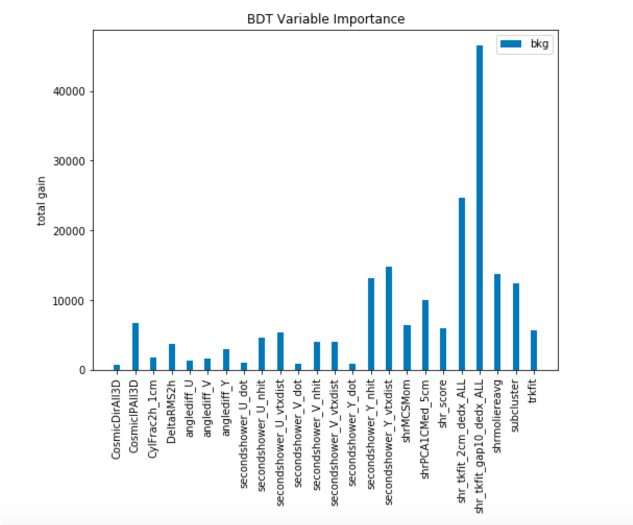
\includegraphics[width=0.7\textwidth]{1e0p/run123_bdt/bdt_importance.png}
\caption{\label{fig:1e0p:bdtvars:RUN3} Relative importance of each variable to BDT.}
\end{center}
\end{figure}


\begin{figure}[H] 
\begin{center}
    \begin{subfigure}[b]{0.45\textwidth}
    \centering
    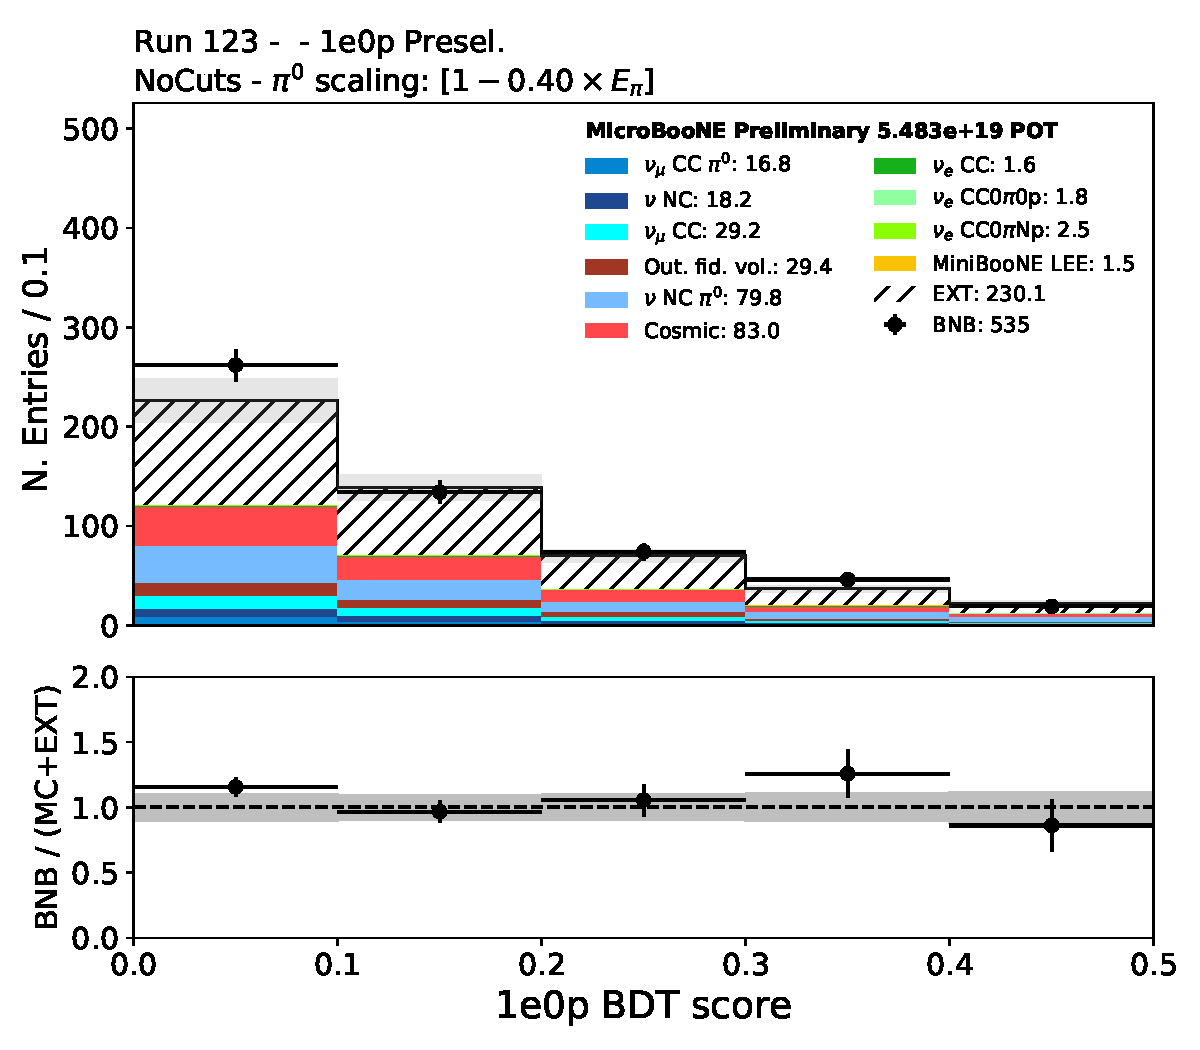
\includegraphics[width=1.00\textwidth]{1e0p/run123_bdt/bkg_score_low_bdt.pdf}
    \caption{\label{fig:1e0p:bdt:bkgscore:slice} Low BDT response (0-0.5).}
    \end{subfigure}
    \begin{subfigure}[b]{0.45\textwidth}
    \centering
    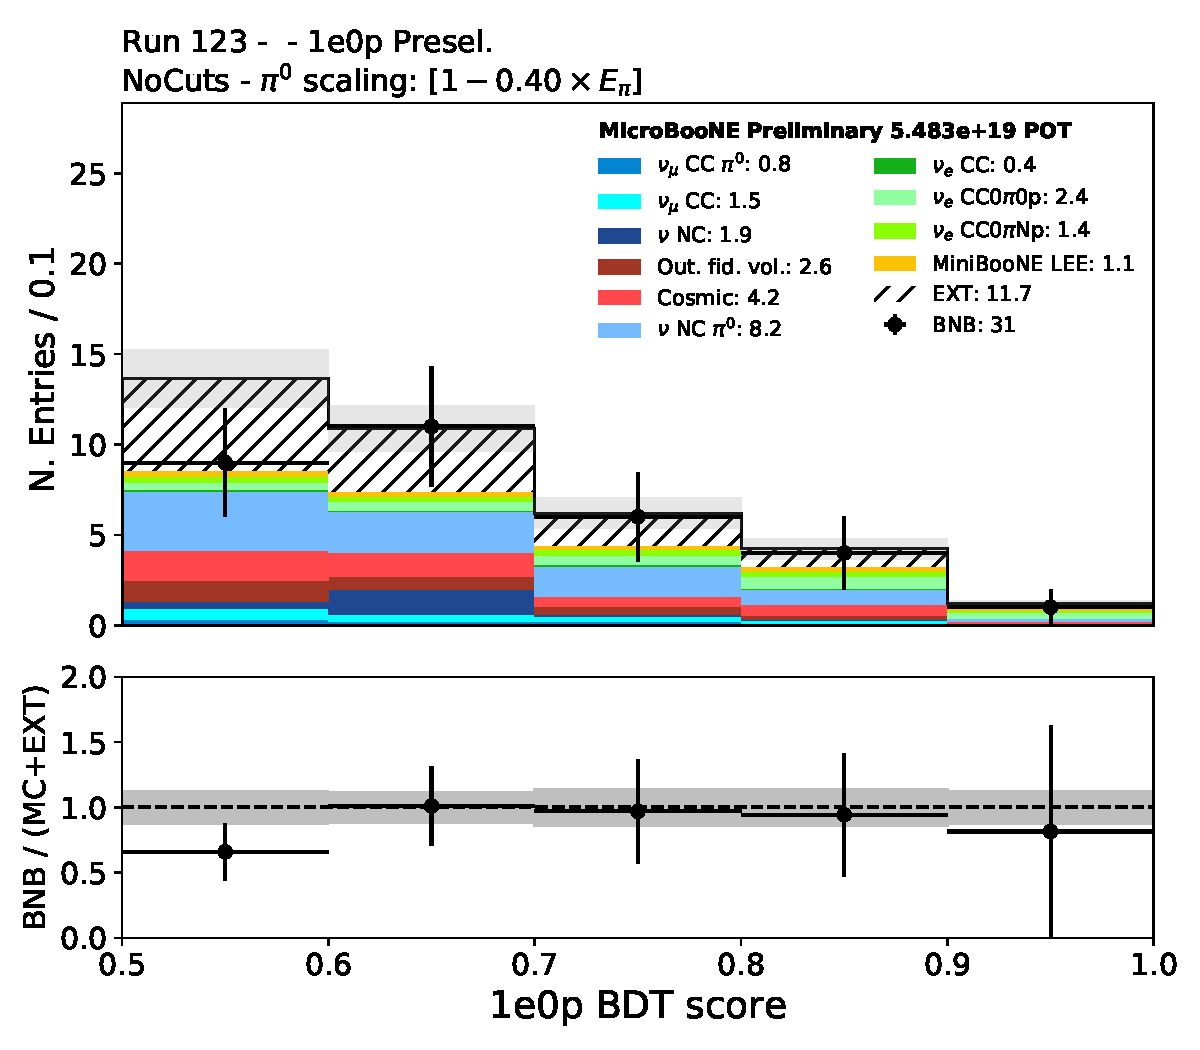
\includegraphics[width=1.00\textwidth]{1e0p/run123_bdt/bkg_score_high_bdt.pdf}
    \caption{\label{fig:1e0p:bdt:bkgscore:presel} High BDT response (0.5-1).}
    \end{subfigure}
\caption{\label{fig:1e0p:bdt:bkgscore} Background BDT response after \zpsel pre-selection.}
\end{center}
\end{figure}


%\begin{figure}[H] 
%\begin{center}
%    \begin{subfigure}[b]{0.45\textwidth}
%    \centering
%    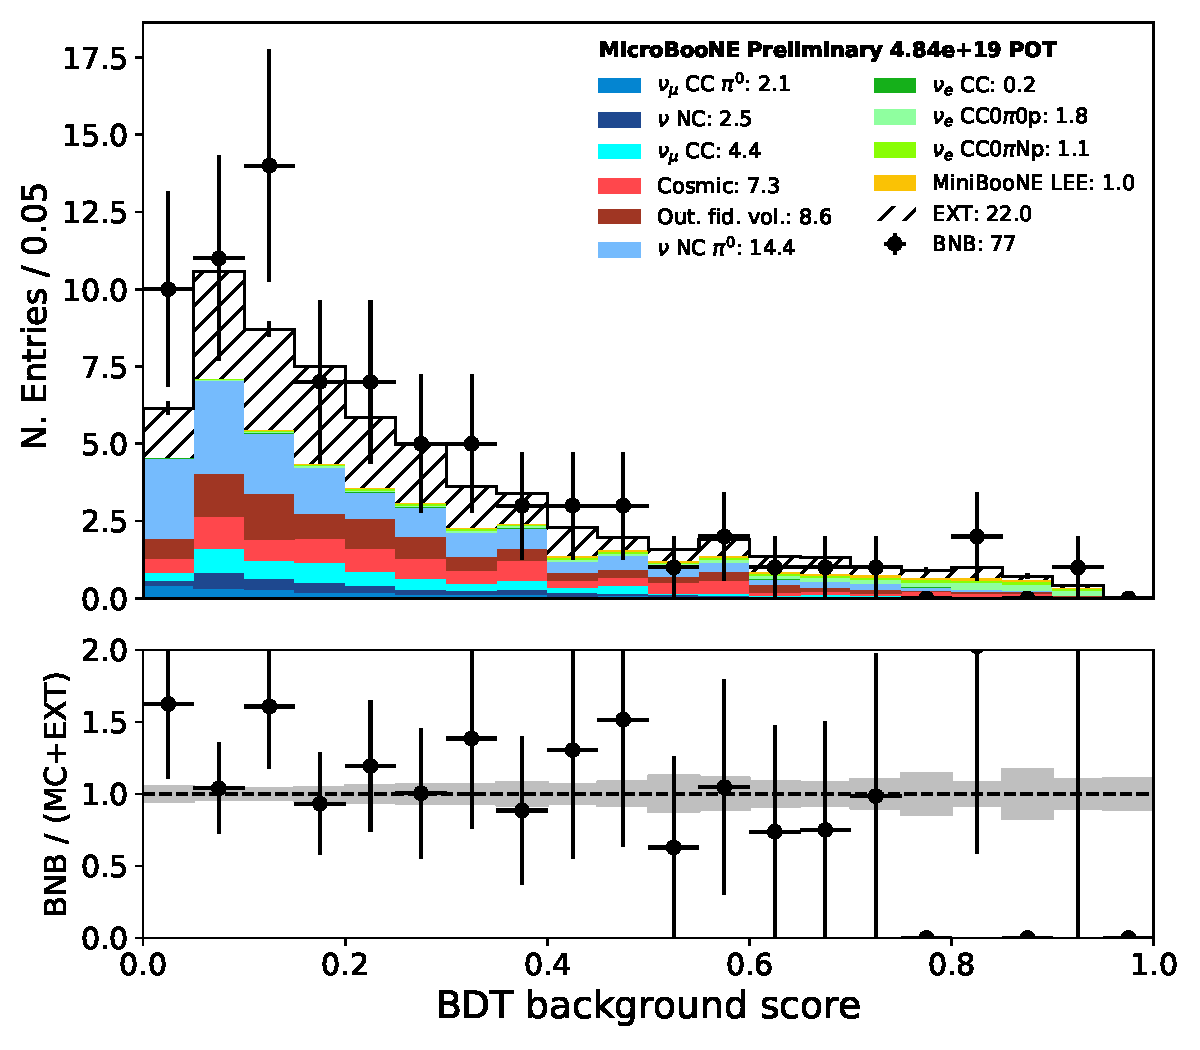
\includegraphics[width=1.00\textwidth]{1e0p/run123_bdt/bkg_score_BDT_R1R2R3_0ploosesel.pdf}
%    \caption{\label{fig:1e0p:bdt:bkgscore:loosenozoom} Full response.}
%    \end{subfigure}
%    \begin{subfigure}[b]{0.45\textwidth}
%    \centering
 %   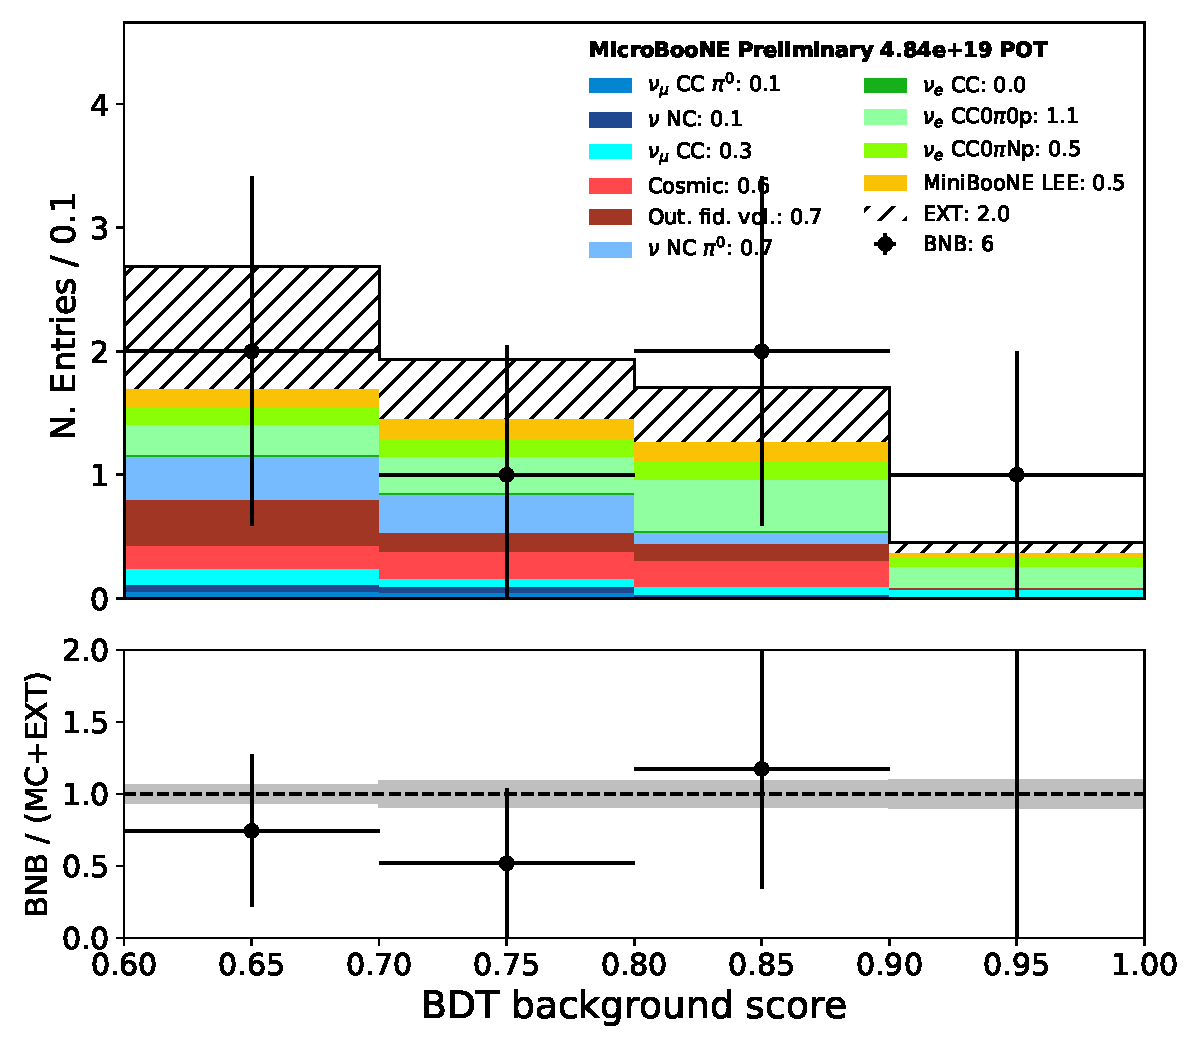
\includegraphics[width=1.00\textwidth]{1e0p/run123_bdt/bkg_score_BDT_R1R2R3_0ploosesel_zoom.pdf}
%    \caption{\label{fig:1e0p:bdt:bkgscore:loosezoom} Zoomed in.}
%    \end{subfigure}
%\caption{\label{fig:1e0p:bdt:loose} BDT response for background BDT after loose selection.}
%\end{center}
%\end{figure}

The data-MC agreement of the BDT response on the Run 1 open data after the \zpsel pre-selection is shown in Fig.~\ref{fig:1e0p:bdt:bkgscore}. The agreement is generally good.  

%The BDT response after the loose selection is shown in Fig.~\ref{fig:1e0p:bdt:loose}.  
%Events above 0.85 in BDT response are selected as signal.  The final BDT selection is the loose cuts defined in Table~\ref{tab:1e0p:loosecut} with the addition of this cut on the BDT response, and a tighter cut on thee second shower search \texttt{secondshower\_Y\_nhit} $<$ 20. 
%This is the selection of events that is used to train the BDT, and these cuts are also applied before cutting on the BDT response for the BDT selection. 
%\textcolor{blue}{I'm confused by this wording}. 

Events above 0.72 in BDT response are selected as signal. The final BDT selection consists of the loose cuts defined in Table~\ref{tab:1e0p:loosecut} with the addition of this cut on the BDT response.

\begin{figure}[H]
\begin{center}
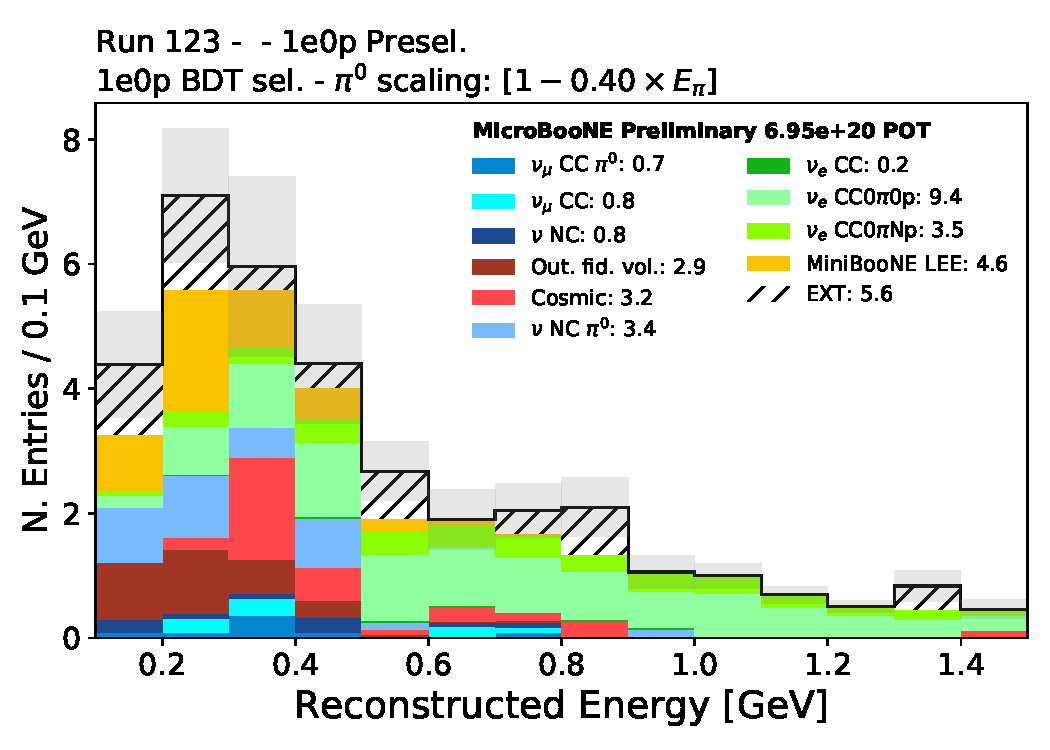
\includegraphics[width=0.65\textwidth]{1e0p/run123_bdt/reco_e_nodata_08052020.pdf}
\caption{\label{fig:1e0p:bdt:loosebdt} BDT selection for \zpsel events, scaled up to the full 10.1e20 POT data set.}
\end{center}
\end{figure}

The reconstructed energy distribution for selected \zpsel events that pass the BDT selection is shown in Fig.~\ref{fig:1e0p:bdt:loosebdt}.  This selection predicts 10 true \zpsel events in the full data set, and is 52\% pure for electron neutrinos and the LEE from 0-2 GeV in reconstructed neutrino energy. 
%This selection predicts 8 true \zpsel events in the full data set, and is 50\% pure for electron neutrinos and the LEE from 0-2 GeV in reconstructed neutrino energy. 
It has a higher efficiency for electron neutrinos and low energy events than the box cut selections presented in Apendix~\ref{app:nueslections:1e0p}.  

%Using the BDT it is also possible to make a selection of \zpsel events that is much more efficient, but only slightly less pure by cutting more loosely on the BDT response.  Fig.~\ref{fig:1e0p:bdt:loosebdt} shows, for example, a cut on the BDT response at 0.72, which is 41\% pure over the same energy region, and about twice as efficient for $\nu_{e}$ and LEE events. 

%Using the BDT it is also possible to make a selection of \zpsel events that is more pure, but less efficient, by cutting more tightly on the BDT response.  Fig.~\ref{fig:1e0p:bdt:RUN3} shows, for example, a cut on the BDT response at 0.85, which is 50\% pure over the same energy region, but about half as efficient for $\nu_{e}$ and LEE events. 

%\begin{figure}[H]
%\begin{center}
%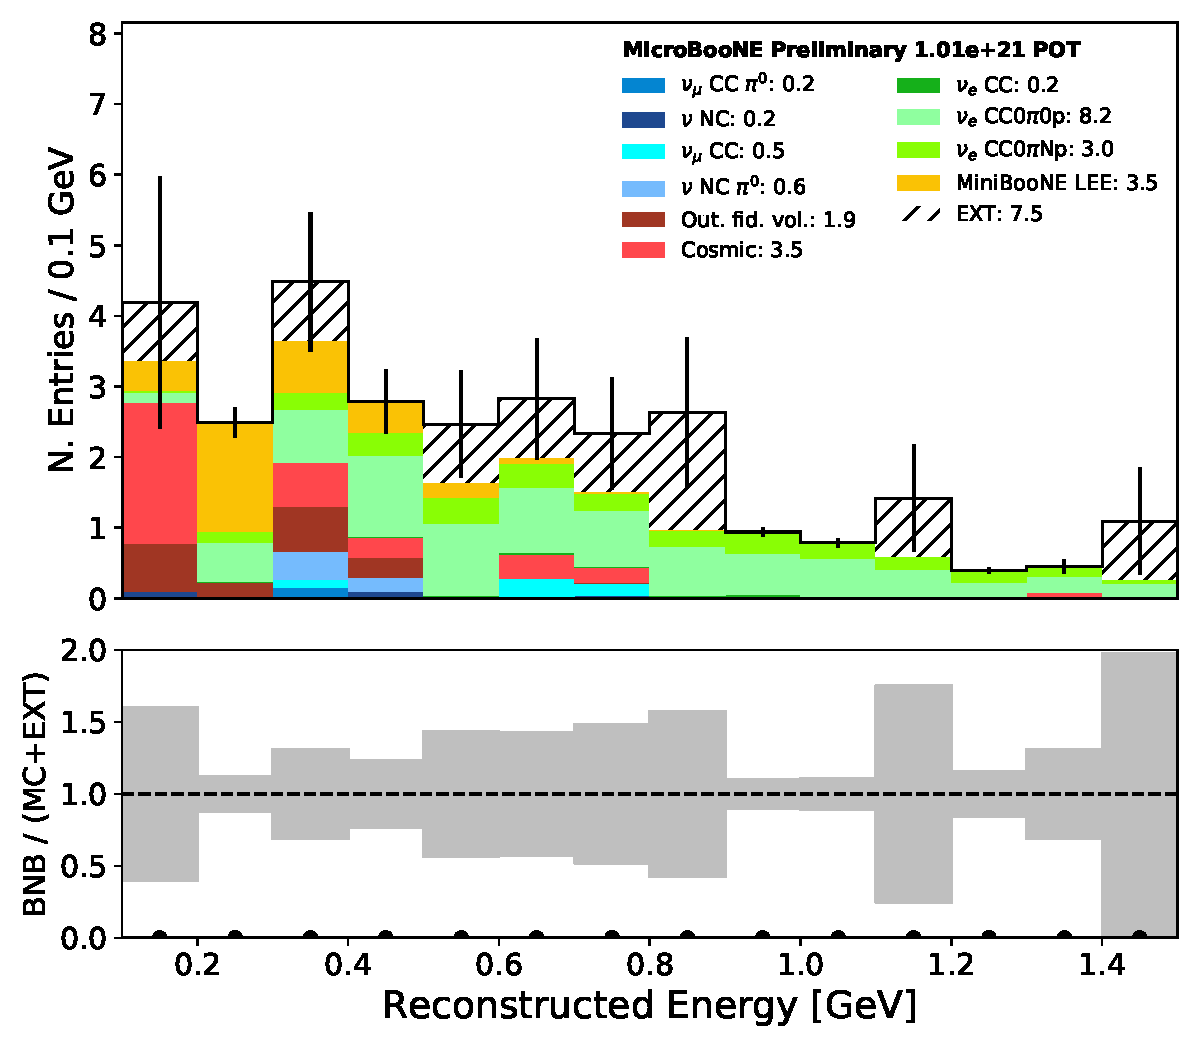
\includegraphics[width=0.45\textwidth]{1e0p/run123_bdt/reco_e_BDT_R1R2R3.pdf}
%\caption{\label{fig:1e0p:bdt:RUN3} BDT selection for \zpsel events, with a tighter cut on the BDT response scaled up to the full 10.1e20 POT data set.}
%\end{center}
%\end{figure}

%The BDT selection in Fig.~\ref{fig:1e0p:bdt:loosebdt} is the nominal BDT selection due to its higher efficiency, but the tighter one in Fig.~\ref{fig:1e0p:bdt:RUN3} could be used if the higher purity is found to have a better impact on the fit and constraint.



\begin{figure}[H]
\begin{center}
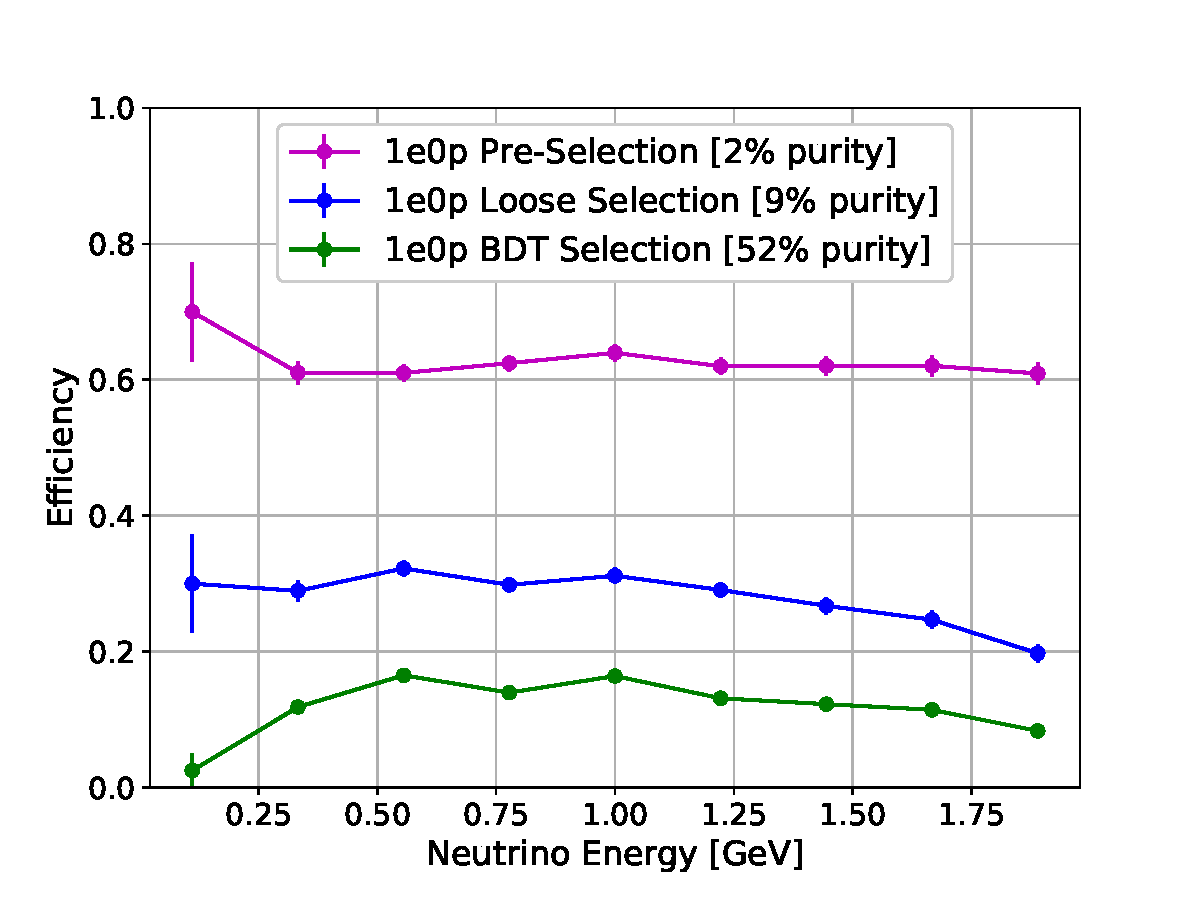
\includegraphics[width=0.65\textwidth]{1e0p/run123_bdt/efficiency08012020.pdf}
\caption{\label{fig:1e0p:eff:RUN3} Efficiency of \zpsel selections.}
\end{center}
\end{figure}

The selection efficiency for the \zpsel cut-based and BDT selections are shown in Fig.~\ref{fig:1e0p:eff:RUN3}.  The main reduction in efficiency in the selection is at pre-selection stage.  The overall efficiency after the BDT selection is about 10\% with a 52\% pure selection, calculated over the energy range from 0-2 GeV.